%============================================================
%  TurtleBot LLM Social Tour Guide — Technical Reference Report
%  Compiled with: pdflatex report.tex (run twice for TOC/refs)
%============================================================
\documentclass[12pt,a4paper]{report}

%------------------------------------------------------------
% Core packages
%------------------------------------------------------------
\usepackage[T1]{fontenc}
\usepackage[utf8]{inputenc}
\usepackage{lmodern}
\usepackage{microtype}
\usepackage[margin=2.5cm]{geometry}
\usepackage{parskip}           % space between paragraphs, no indent
\usepackage{setspace}
\onehalfspacing

%------------------------------------------------------------
% Colour & graphics
%------------------------------------------------------------
\usepackage[dvipsnames,table]{xcolor}
\usepackage{graphicx}
\usepackage{tikz}
\usetikzlibrary{shapes.geometric, arrows.meta, positioning, fit, backgrounds, calc}

%------------------------------------------------------------
% Hyperlinks
%------------------------------------------------------------
\usepackage[
  colorlinks=true,
  linkcolor=RoyalBlue,
  urlcolor=RoyalBlue,
  citecolor=RoyalBlue,
  bookmarks=true,
  bookmarksopen=true,
  pdfauthor={Karan},
  pdftitle={TurtleBot LLM Social Tour Guide — Technical Reference Report},
]{hyperref}

%------------------------------------------------------------
% Code listings
%------------------------------------------------------------
\usepackage{listings}
\usepackage{lstautogobble}

\definecolor{codebg}{HTML}{F5F5F5}
\definecolor{codeframe}{HTML}{CCCCCC}
\definecolor{codestring}{HTML}{008800}
\definecolor{codekw}{HTML}{0000AA}
\definecolor{codecomment}{HTML}{888888}

\lstdefinestyle{bashstyle}{
  language=bash,
  backgroundcolor=\color{codebg},
  frame=single,
  rulecolor=\color{codeframe},
  basicstyle=\ttfamily\footnotesize,
  keywordstyle=\color{codekw}\bfseries,
  stringstyle=\color{codestring},
  commentstyle=\color{codecomment}\itshape,
  breaklines=true,
  autogobble=true,
  showstringspaces=false,
  numbers=left,
  numberstyle=\tiny\color{gray},
  numbersep=8pt,
  xleftmargin=16pt,
  framexleftmargin=16pt,
}

\lstdefinestyle{pythonstyle}{
  language=Python,
  backgroundcolor=\color{codebg},
  frame=single,
  rulecolor=\color{codeframe},
  basicstyle=\ttfamily\footnotesize,
  keywordstyle=\color{codekw}\bfseries,
  stringstyle=\color{codestring},
  commentstyle=\color{codecomment}\itshape,
  breaklines=true,
  autogobble=true,
  showstringspaces=false,
  numbers=left,
  numberstyle=\tiny\color{gray},
  numbersep=8pt,
  xleftmargin=16pt,
  framexleftmargin=16pt,
}

\lstdefinestyle{xmlstyle}{
  language=XML,
  backgroundcolor=\color{codebg},
  frame=single,
  rulecolor=\color{codeframe},
  basicstyle=\ttfamily\footnotesize,
  keywordstyle=\color{codekw}\bfseries,
  stringstyle=\color{codestring},
  commentstyle=\color{codecomment}\itshape,
  breaklines=true,
  autogobble=true,
  showstringspaces=false,
  xleftmargin=8pt,
  framexleftmargin=8pt,
}

%------------------------------------------------------------
% Tables
%------------------------------------------------------------
\usepackage{booktabs}
\usepackage{longtable}
\usepackage{tabularx}
\usepackage{multirow}
\usepackage{array}

\newcolumntype{L}[1]{>{\raggedright\arraybackslash}p{#1}}
\newcolumntype{C}[1]{>{\centering\arraybackslash}p{#1}}

%------------------------------------------------------------
% Boxes / callouts
%------------------------------------------------------------
\usepackage{tcolorbox}
\tcbuselibrary{skins, breakable, listings}

\tcbset{
  notebox/.style={
    enhanced,
    breakable,
    colback=blue!5,
    colframe=RoyalBlue!70,
    fonttitle=\bfseries,
    left=6pt, right=6pt, top=4pt, bottom=4pt,
  },
  warnbox/.style={
    enhanced,
    breakable,
    colback=orange!8,
    colframe=orange!80!black,
    fonttitle=\bfseries,
    left=6pt, right=6pt, top=4pt, bottom=4pt,
  },
  tipbox/.style={
    enhanced,
    breakable,
    colback=green!6,
    colframe=green!60!black,
    fonttitle=\bfseries,
    left=6pt, right=6pt, top=4pt, bottom=4pt,
  },
}

%------------------------------------------------------------
% Misc utilities
%------------------------------------------------------------
\usepackage{enumitem}
\usepackage{fancyhdr}
\usepackage{titlesec}
\usepackage{float}
\usepackage{caption}
\usepackage{subcaption}
\usepackage{amsmath}

%------------------------------------------------------------
% Header / footer
%------------------------------------------------------------
\pagestyle{fancy}
\fancyhf{}
\fancyhead[L]{\small\nouppercase{\leftmark}}
\fancyhead[R]{\small TurtleBot LLM Social Tour Guide}
\fancyfoot[C]{\thepage}
\renewcommand{\headrulewidth}{0.4pt}

%------------------------------------------------------------
% Chapter / section styling
%------------------------------------------------------------
\titleformat{\chapter}[block]
  {\normalfont\LARGE\bfseries\color{RoyalBlue}}
  {\thechapter.}{12pt}{}
  [\vspace{-4pt}\color{RoyalBlue}\rule{\linewidth}{0.6pt}\vspace{4pt}]

\titleformat{\section}
  {\normalfont\large\bfseries\color{black!80}}
  {\thesection}{8pt}{}

\titleformat{\subsection}
  {\normalfont\normalsize\bfseries}
  {\thesubsection}{6pt}{}

%------------------------------------------------------------
% Convenience commands
%------------------------------------------------------------
\newcommand{\pkg}[1]{\texttt{\color{RoyalBlue}#1}}
\newcommand{\topic}[1]{\texttt{\color{purple!80!black}#1}}
\newcommand{\file}[1]{\texttt{\color{black!70}#1}}
\newcommand{\node}[1]{\texttt{\color{Maroon}#1}}
\newcommand{\kw}[1]{\textbf{#1}}

%============================================================
\begin{document}
%============================================================

%------------------------------------------------------------
% TITLE PAGE
%------------------------------------------------------------
\begin{titlepage}
  \centering
  \vspace*{2cm}

  {\color{RoyalBlue}\rule{\linewidth}{2pt}}
  \vspace{0.6cm}

  {\Huge\bfseries TurtleBot LLM Social Tour Guide}\\[0.4cm]
  {\Large\bfseries Technical Reference Report}\\[0.2cm]
  {\large Complete Package Documentation and Architecture Guide}

  \vspace{0.4cm}
  {\color{RoyalBlue}\rule{\linewidth}{2pt}}

  \vspace{1.8cm}

  {\large
    \begin{tabular}{ll}
      \textbf{Workspace root:}  & \texttt{/home/karan/in\_ws}              \\[4pt]
      \textbf{ROS version:}     & ROS~2 (Humble / Iron compatible)          \\[4pt]
      \textbf{Robot platform:}  & TurtleBot~3 (Burger / Waffle / Waffle Pi) \\[4pt]
      \textbf{LLM backend:}     & Ollama (local, offline) — Qwen 2.5        \\[4pt]
      \textbf{Document date:}   & May 2026                                  \\
    \end{tabular}
  }

  \vspace{2cm}

  \begin{tcolorbox}[notebox, title=About this Document]
    This report is a \emph{complete} technical reference for the
    \pkg{turtlebot\_llm\_control} and \pkg{turtlebot\_social\_guide}
    ROS~2 packages.  It is intended to be self-contained: a reader
    who has never seen the code before should be able to understand
    the system architecture, data flow, module responsibilities, and
    operational procedures after reading this document from start to
    finish.
  \end{tcolorbox}

  \vfill
  {\small Generated from workspace summary $\cdot$ \texttt{/home/karan/in\_ws/summary.md}}
\end{titlepage}

%------------------------------------------------------------
% TABLE OF CONTENTS
%------------------------------------------------------------
\tableofcontents
\clearpage

%============================================================
\chapter{Introduction and Motivation}
\label{ch:intro}
%============================================================

\section{Project Overview}

This workspace implements a \kw{social tour guide robot} built on top of the
TurtleBot~3 mobile platform and the ROS~2 middleware framework.  The robot is
capable of:

\begin{itemize}[leftmargin=2em]
  \item Listening to natural-language voice commands from visitors.
  \item Interpreting commands using both rule-based heuristics and a cloud
        Large Language Model (LLM) API.
  \item Autonomously navigating through a mapped environment using the
        Nav2 navigation stack.
  \item Recording and replaying tour routes (sequences of waypoints).
  \item Maintaining a local knowledge database that stores points of interest
        and answers factual questions posed by visitors.
  \item Following a person using colour-blob tracking from a camera feed.
  \item Synthesising spoken responses delivered through onboard speakers.
\end{itemize}

The system is designed so that \emph{no internet connection is strictly
required}: if no LLM API key is configured, every speech command falls back to
a deterministic rule-based parser, guaranteeing baseline operation in
offline or air-gapped environments.

\section{Why ROS 2?}

ROS~2 (Robot Operating System 2) is an open-source middleware framework that
provides:

\begin{itemize}[leftmargin=2em]
  \item \textbf{Publisher--subscriber messaging} over DDS (Data Distribution
        Service), enabling nodes to exchange typed messages without knowing
        about one another's internal implementation.
  \item \textbf{Service calls} (synchronous request--response) and
        \textbf{action servers} (long-running tasks with feedback), both of
        which are heavily used here.
  \item \textbf{Launch files} (Python-based) for declarative multi-node
        startup.
  \item \textbf{colcon} build system integration.
  \item Compatibility with TurtleBot~3 driver packages and the Nav2
        navigation stack.
\end{itemize}

\begin{tcolorbox}[notebox, title=Key Concept: Node]
  In ROS~2, a \emph{node} is an independently running process.  Nodes
  communicate by publishing messages to \emph{topics} (named channels)
  or by calling \emph{services}.  This architecture allows any node to
  be replaced, restarted, or scaled independently of the others.
\end{tcolorbox}

\section{Scope of This Document}

This document covers:

\begin{enumerate}[leftmargin=2em]
  \item Workspace layout and directory structure.
  \item Detailed descriptions of every Python module and ROS~2 node.
  \item Full data-flow diagrams for the speech, navigation, tour, and
        knowledge subsystems.
  \item Build, install, and launch procedures.
  \item LLM integration details, including API key management and
        fallback behaviour.
  \item Complete dependency tables.
  \item A recommended reading order for developers new to the codebase.
\end{enumerate}

%============================================================
\chapter{Workspace Layout}
\label{ch:layout}
%============================================================

\section{Top-Level Directory Structure}

The workspace root is \texttt{/home/karan/in\_ws}.  After a clean build the
directory tree looks like this:

\begin{lstlisting}[style=bashstyle, caption={Top-level workspace directory tree}]
/home/karan/in_ws/
├── src/
│   ├── turtlebot_LLM_control/        # Main LLM-driven control package
│   └── turtlebot_social_guide/       # Supporting social-guide package
├── build/                            # colcon build artefacts (generated)
├── install/                          # Installed package overlays (generated)
├── log/                              # colcon build logs (generated)
└── summary.md                        # Human-readable workspace summary
\end{lstlisting}

\begin{tcolorbox}[warnbox, title=Important: Generated Directories]
  The \texttt{build/}, \texttt{install/}, and \texttt{log/} directories are
  \emph{generated} by \texttt{colcon build} and should \textbf{never} be
  committed to version control.  They are safe to delete; re-running
  \texttt{colcon build} recreates them.
\end{tcolorbox}

\section{Package: \texttt{turtlebot\_LLM\_control}}

\begin{lstlisting}[style=bashstyle, caption={\texttt{turtlebot\_LLM\_control} internal layout}]
src/turtlebot_LLM_control/
├── package.xml                        # ROS 2 package manifest
├── setup.py                           # Python package installer / entry points
├── setup.cfg                          # Build configuration
├── README.md                          # User-facing documentation
├── GUIDE.md                           # Developer setup / workflow guide
│
├── launch/
│   ├── bringup.launch.py              # Core stack launcher (hw + sim)
│   └── sim_pillar_nav_demo.launch.py  # Full simulation demo launcher
│
├── config/
│   └── demo_nav2/
│       ├── burger.yaml                # Nav2 params for Burger model
│       ├── waffle.yaml                # Nav2 params for Waffle model
│       └── waffle_pi.yaml             # Nav2 params for Waffle Pi model
│
├── maps/
│   └── demo/
│       ├── map.yaml                   # Map metadata
│       └── map.pgm                    # Occupancy grid image
│
├── rviz/
│   └── tb3_navigation2.rviz          # RViz2 visualisation config
│
└── turtlebot_llm_control/            # Python package (importable module)
    ├── __init__.py
    ├── api.key.example               # Example LLM API key file
    ├── audio_utils.py
    ├── behavior_tree.py
    ├── bt_orchestrator_node.py
    ├── follow_me_node.py
    ├── knowledge_editor.py
    ├── knowledge_overlay_node.py
    ├── knowledge_store.py
    ├── llm_dialogue.py
    ├── llm_intent_test.py
    ├── models.py
    ├── predefined_commands.py
    ├── sim_initial_pose_node.py
    ├── speech_command_node.py
    ├── speech_debug_node.py
    ├── speech_parser.py
    ├── speech_response_node.py
    ├── speech_to_text_node.py
    ├── tour_recording_manager.py
    ├── tour_teleop_session.py
    └── wake_word.py
\end{lstlisting}

\section{Package: \texttt{turtlebot\_social\_guide}}

\begin{lstlisting}[style=bashstyle, caption={\texttt{turtlebot\_social\_guide} internal layout}]
src/turtlebot_social_guide/
└── src/
    ├── tour_manager/
    │   ├── package.xml
    │   ├── setup.py
    │   ├── setup.cfg
    │   ├── launch/
    │   │   └── tour_manager_launch.py
    │   └── tour_manager/
    │       ├── __init__.py
    │       ├── tour_saver.py
    │       ├── tour_manager_service.py
    │       └── waypoint_visualizer.py
    │
    ├── speech_locomotion_interface/
    │   ├── package.xml
    │   ├── setup.py
    │   └── speech_locomotion_interface/
    │       ├── __init__.py
    │       └── speech_listener.py
    │
    ├── social_robot_interfaces/
    │   ├── package.xml
    │   └── srv/
    │       └── Tours.srv              # Custom ROS 2 service definition
    │
    └── robot_tour/
        ├── package.xml
        ├── CMakeLists.txt             # C++ build rules
        ├── plugins.xml                # Plugin export declaration
        ├── src/
        │   └── tour_guide.cpp
        └── plugins/
            └── talk_at_waypoint.cpp
\end{lstlisting}

%============================================================
\chapter{Package Descriptions}
\label{ch:packages}
%============================================================

\section{\texttt{turtlebot\_llm\_control} — The Brain}
\label{sec:llm_control}

This is the \emph{primary} package in the workspace.  It owns the complete
speech-to-action pipeline: from raw audio capture, through intent
classification, down to Nav2 action goals and spoken responses.  Every
subsystem described in later chapters (speech, navigation, tour, knowledge) has
its implementation here.

\subsection{Package Manifest (\texttt{package.xml})}

The \file{package.xml} file declares the ROS~2 package identity and its
dependencies.  An abridged representation is shown below:

\begin{lstlisting}[style=xmlstyle, caption={Key sections of \texttt{package.xml}}]
<package format="3">
  <name>turtlebot_llm_control</name>
  <version>0.1.0</version>
  <buildtool_depend>ament_python</buildtool_depend>

  <!-- Core ROS 2 communication -->
  <depend>rclpy</depend>
  <depend>std_msgs</depend>
  <depend>geometry_msgs</depend>
  <depend>nav_msgs</depend>
  <depend>nav2_msgs</depend>
  <depend>sensor_msgs</depend>
  <depend>action_msgs</depend>
  <depend>tf2_ros</depend>
  <depend>tf_transformations</depend>
  <depend>visualization_msgs</depend>

  <!-- Launch infrastructure -->
  <depend>launch</depend>
  <depend>launch_ros</depend>
  <depend>ament_index_python</depend>

  <!-- Runtime: social guide sub-packages -->
  <exec_depend>speech_locomotion_interface</exec_depend>
  <exec_depend>tour_manager</exec_depend>
</package>
\end{lstlisting}

\subsection{Python Entry Points (\texttt{setup.py})}

\texttt{setup.py} registers every node as a named console script so that
\texttt{ros2~run} can find it:

\begin{lstlisting}[style=pythonstyle, caption={Excerpt showing entry-point registration pattern}]
setup(
    name='turtlebot_llm_control',
    packages=find_packages(),
    entry_points={
        'console_scripts': [
            'bt_orchestrator_node   = turtlebot_llm_control.bt_orchestrator_node:main',
            'speech_to_text_node    = turtlebot_llm_control.speech_to_text_node:main',
            'speech_command_node    = turtlebot_llm_control.speech_command_node:main',
            'speech_response_node   = turtlebot_llm_control.speech_response_node:main',
            'speech_debug_node      = turtlebot_llm_control.speech_debug_node:main',
            'follow_me_node         = turtlebot_llm_control.follow_me_node:main',
            'knowledge_editor       = turtlebot_llm_control.knowledge_editor:main',
            'knowledge_overlay_node = turtlebot_llm_control.knowledge_overlay_node:main',
            'tour_recording_manager = turtlebot_llm_control.tour_recording_manager:main',
            'wake_word               = turtlebot_llm_control.wake_word:main',
            # ... and more
        ],
    },
)
\end{lstlisting}

\section{\texttt{turtlebot\_social\_guide} — The Support Stack}
\label{sec:social_guide}

This package is a \emph{dependency} of the main control package.  It contains
three sub-packages and one C++ plugin package:

\begin{description}[leftmargin=2em, style=nextline]
  \item[\pkg{tour\_manager}]
    A ROS~2 Python package that exposes a \emph{service server} for tour
    retrieval and saving, a \emph{tour saver node} that responds to save
    commands, and a \emph{waypoint visualiser} that publishes
    \texttt{visualization\_msgs/MarkerArray} messages.

  \item[\pkg{speech\_locomotion\_interface}]
    A thin ROS~2 Python node (\node{speech\_listener}) that listens on
    \topic{/speech/intent} and directly drives the robot using the
    \texttt{nav2\_simple\_commander} Python API.  This provides a
    \emph{fallback} navigation path that bypasses the behaviour tree.

  \item[\pkg{social\_robot\_interfaces}]
    A pure-interface package containing only \file{Tours.srv}, the custom
    ROS~2 service definition used by the tour manager.  Separating interface
    definitions into their own package is ROS~2 best practice because it allows
    any downstream package to depend on the interface without pulling in
    implementation code.

  \item[\pkg{robot\_tour}]
    A C++ package that implements a Nav2 Behaviour Tree plugin
    (\texttt{TalkAtWaypoint}) and a tour guide executable.  This plugin fires
    a callback each time the robot reaches a waypoint, allowing speech
    synthesis to be triggered at specific locations on a tour route.
\end{description}

%============================================================
\chapter{Node Reference}
\label{ch:nodes}
%============================================================

This chapter provides a detailed description of every ROS~2 node in the
workspace, including its subscriptions, publications, services, action clients,
and responsibilities.

\section{Speech Pipeline Nodes}

\subsection{\node{speech\_to\_text\_node}}
\label{sub:stt}

\textbf{File:} \file{turtlebot\_llm\_control/speech\_to\_text\_node.py}

\textbf{Purpose:} The entry point to the speech pipeline.  It converts either
real microphone audio (via the \texttt{speech\_recognition} library) or
injected mock text into a plain UTF-8 string and publishes it on
\topic{/speech/text}.  Wake-word gating (see Section~\ref{sub:wake}) is
integrated: the node will not publish text until the wake word has been
detected.

\begin{table}[H]
  \centering
  \caption{Topics for \texttt{speech\_to\_text\_node}}
  \begin{tabularx}{\linewidth}{L{3cm} L{4.5cm} X}
    \toprule
    \textbf{Direction} & \textbf{Topic} & \textbf{Description} \\
    \midrule
    Publishes   & \topic{/speech/text}              & Recognised speech as a \texttt{std\_msgs/String} \\
    Publishes   & \topic{/speech\_to\_text/status}  & Node health / state as \texttt{std\_msgs/String} \\
    Subscribes  & \topic{/speech/mock\_text}        & Inject text without a microphone (testing) \\
    \bottomrule
  \end{tabularx}
\end{table}

\subsection{\node{speech\_command\_node}}
\label{sub:scn}

\textbf{File:} \file{turtlebot\_llm\_control/speech\_command\_node.py}

\textbf{Purpose:} Bridges raw transcribed text and structured robot intents.
It calls \texttt{llm\_dialogue.generate\_llm\_token()} (or the rule-based
\texttt{speech\_parser} fallback) and publishes a JSON-encoded intent message.

\begin{table}[H]
  \centering
  \caption{Topics for \texttt{speech\_command\_node}}
  \begin{tabularx}{\linewidth}{L{3cm} L{4.5cm} X}
    \toprule
    \textbf{Direction} & \textbf{Topic} & \textbf{Description} \\
    \midrule
    Subscribes  & \topic{/speech/text}    & Receives transcribed text \\
    Publishes   & \topic{/speech/intent}  & Structured intent JSON as \texttt{std\_msgs/String} \\
    \bottomrule
  \end{tabularx}
\end{table}

The intent JSON schema is:

\begin{lstlisting}[style=pythonstyle, caption={Intent JSON schema produced by \texttt{speech\_command\_node}}]
{
  "intent":   "<string>",   # See intent table below
  "label":    "<string>",   # Human-readable action label
  "location": "<string>",   # Target location name (may be null)
  "response": "<string>",   # Suggested spoken response
  "metadata": {}            # Optional extra fields
}
\end{lstlisting}

\begin{table}[H]
  \centering
  \caption{Allowed intent values}
  \begin{tabularx}{\linewidth}{L{4cm} X}
    \toprule
    \textbf{Intent} & \textbf{Meaning} \\
    \midrule
    \texttt{navigate}          & Navigate to a named location \\
    \texttt{tour\_start}       & Begin a pre-recorded tour \\
    \texttt{tour\_stop}        & Abort the current tour \\
    \texttt{record\_start}     & Begin recording a new route \\
    \texttt{record\_stop}      & Stop recording and save the route \\
    \texttt{manual\_override}  & Enable/disable manual teleoperation \\
    \texttt{follow\_me}        & Enable/disable person-following mode \\
    \texttt{explain}           & Answer a knowledge question \\
    \texttt{no\_action}        & Utterance is not a command \\
    \bottomrule
  \end{tabularx}
\end{table}

\subsection{\node{speech\_response\_node}}
\label{sub:srn}

\textbf{File:} \file{turtlebot\_llm\_control/speech\_response\_node.py}

\textbf{Purpose:} Converts text responses into audible speech using the
operating system's text-to-speech (TTS) engine.  The node tries the following
TTS backends in order: \texttt{spd-say} (Linux Speech Dispatcher),
\texttt{espeak}, and the macOS \texttt{say} command.

\begin{table}[H]
  \centering
  \caption{Topics for \texttt{speech\_response\_node}}
  \begin{tabularx}{\linewidth}{L{3cm} L{4.5cm} X}
    \toprule
    \textbf{Direction} & \textbf{Topic} & \textbf{Description} \\
    \midrule
    Subscribes & \topic{/speech/response} & Text string to synthesise \\
    \bottomrule
  \end{tabularx}
\end{table}

\subsection{\node{speech\_debug\_node}}
\label{sub:sdn}

\textbf{File:} \file{turtlebot\_llm\_control/speech\_debug\_node.py}

\textbf{Purpose:} An observability node that aggregates messages from every
speech-pipeline topic and re-publishes a combined diagnostic string on
\topic{/speech/debug}.  Useful for monitoring the full pipeline state from a
single \texttt{ros2 topic echo} command.

\begin{table}[H]
  \centering
  \caption{Topics for \texttt{speech\_debug\_node}}
  \begin{tabularx}{\linewidth}{L{3cm} L{4.5cm} X}
    \toprule
    \textbf{Direction} & \textbf{Topic} & \textbf{Description} \\
    \midrule
    Subscribes & \topic{/speech\_to\_text/status} & STT node status \\
    Subscribes & \topic{/speech/text}             & Transcribed text \\
    Subscribes & \topic{/speech/intent}            & Parsed intent JSON \\
    Subscribes & \topic{/speech/response}          & TTS response text \\
    Publishes  & \topic{/speech/debug}             & Aggregated diagnostic string \\
    \bottomrule
  \end{tabularx}
\end{table}

\subsection{\node{wake\_word} (module)}
\label{sub:wake}

\textbf{File:} \file{turtlebot\_llm\_control/wake\_word.py}

\textbf{Purpose:} This module (not a standalone node; embedded inside
\node{speech\_to\_text\_node}) provides two functions:
(1)~\emph{wake-word detection} — the robot only begins processing speech after
hearing a designated activation phrase; and (2)~\emph{emergency stop logic}
— certain phrases (e.g., ``stop'', ``emergency'') publish a zero-velocity
command directly, bypassing the behaviour tree, to halt the robot immediately.

\section{Orchestration Node}

\subsection{\node{bt\_orchestrator\_node}}
\label{sub:bt}

\textbf{File:} \file{turtlebot\_llm\_control/bt\_orchestrator\_node.py}

\textbf{Purpose:} The \emph{central decision hub} of the robot.  It consumes
intent messages produced by \node{speech\_command\_node} and dispatches the
appropriate low-level actions.  It is built on top of a \emph{custom behaviour
tree} implementation in \file{behavior\_tree.py}.

\textbf{Responsibilities:}
\begin{itemize}[leftmargin=2em]
  \item Receiving structured intent messages.
  \item Sending \texttt{NavigateToPose} action goals to the Nav2 action server.
  \item Enabling or disabling tour replay, manual override, and follow-me modes
        by publishing control flags.
  \item Commanding tour recording start/stop.
  \item Triggering the LLM for personalised spoken responses.
  \item Publishing tour status updates.
\end{itemize}

\begin{table}[H]
  \centering
  \caption{Complete topic table for \texttt{bt\_orchestrator\_node}}
  \begin{tabularx}{\linewidth}{L{3cm} L{5.5cm} X}
    \toprule
    \textbf{Direction} & \textbf{Topic / Action} & \textbf{Type / Description} \\
    \midrule
    Subscribes  & \topic{/speech/intent}           & Intent JSON from \node{speech\_command\_node} \\
    \midrule
    Publishes   & \topic{/speech/response}         & \texttt{std\_msgs/String} — spoken reply \\
    Publishes   & \topic{/tour/status}             & \texttt{std\_msgs/String} — tour state \\
    Publishes   & \topic{/route/record}            & \texttt{std\_msgs/Bool} — start/stop recording \\
    Publishes   & \topic{/save\_tour\_command}     & \texttt{std\_msgs/String} — save trigger \\
    Publishes   & \topic{/route/replay}            & \texttt{std\_msgs/String} — replay trigger \\
    Publishes   & \topic{/reactive\_nav/control}   & \texttt{std\_msgs/Bool} — reactive nav flag \\
    Publishes   & \topic{/manual\_override/control}& \texttt{std\_msgs/Bool} — manual mode flag \\
    Publishes   & \topic{/follow\_me/control}      & \texttt{std\_msgs/Bool} — follow-me flag \\
    \midrule
    Action Client & \topic{/navigate\_to\_pose}    & \texttt{nav2\_msgs/NavigateToPose} — sends goals to Nav2 \\
    \bottomrule
  \end{tabularx}
\end{table}

\subsection{Behaviour Tree (\texttt{behavior\_tree.py})}

\textbf{File:} \file{turtlebot\_llm\_control/behavior\_tree.py}

This module provides a \emph{lightweight} behaviour tree framework used
exclusively by \node{bt\_orchestrator\_node}.  A behaviour tree is a
hierarchical control structure where each \emph{node} is either:

\begin{description}[leftmargin=2em]
  \item[Leaf node (Action)] Performs a concrete operation (e.g., send a Nav2
    goal, publish a message) and returns \texttt{SUCCESS}, \texttt{FAILURE},
    or \texttt{RUNNING}.
  \item[Sequence node] Ticks child nodes left-to-right; returns \texttt{FAILURE}
    on the first child failure.
  \item[Selector/Fallback node] Ticks child nodes left-to-right; returns
    \texttt{SUCCESS} on the first child success.
\end{description}

Using a behaviour tree instead of a flat \texttt{if/elif} chain makes it easy
to add, remove, or re-order behaviours without restructuring the entire
decision logic.

\section{Navigation and Sensing Nodes}

\subsection{\node{sim\_initial\_pose\_node}}
\label{sub:siposn}

\textbf{File:} \file{turtlebot\_llm\_control/sim\_initial\_pose\_node.py}

\textbf{Purpose:} In simulation the AMCL localiser requires an initial pose
estimate before it can track the robot's position.  This node publishes a
hard-coded (or parameter-configured) \texttt{geometry\_msgs/PoseWithCovarianceStamped}
message to \topic{/initialpose} once on startup, unblocking the Nav2 stack.

\subsection{\node{follow\_me\_node}}
\label{sub:fmn}

\textbf{File:} \file{turtlebot\_llm\_control/follow\_me\_node.py}

\textbf{Purpose:} Implements a visual person-following behaviour using
colour-blob tracking.  The node subscribes to the robot's camera, identifies
a coloured target in each frame (using OpenCV), computes the angular and linear
error between the robot centre and the target centroid, and publishes
proportional-control velocity commands.

\begin{table}[H]
  \centering
  \caption{Topics for \texttt{follow\_me\_node}}
  \begin{tabularx}{\linewidth}{L{3cm} L{5.5cm} X}
    \toprule
    \textbf{Direction} & \textbf{Topic} & \textbf{Type / Description} \\
    \midrule
    Subscribes & \topic{/follow\_me/control}               & \texttt{std\_msgs/Bool} — enable/disable \\
    Subscribes & \topic{/camera/image\_raw}                & \texttt{sensor\_msgs/Image} — raw camera frames \\
    Subscribes & \topic{/camera/image\_raw/compressed}     & \texttt{sensor\_msgs/CompressedImage} — compressed frames \\
    \midrule
    Publishes  & \topic{/cmd\_vel}                         & \texttt{geometry\_msgs/Twist} — velocity command \\
    Publishes  & \topic{/follow\_me/status}                & \texttt{std\_msgs/String} — tracking status \\
    Publishes  & \topic{/follow\_me/debug/compressed}      & \texttt{sensor\_msgs/CompressedImage} — annotated frame \\
    \bottomrule
  \end{tabularx}
\end{table}

\section{Tour and Route Management Nodes}

\subsection{\node{tour\_recording\_manager}}
\label{sub:trm}

\textbf{File:} \file{turtlebot\_llm\_control/tour\_recording\_manager.py}

\textbf{Purpose:} Records the robot's pose trajectory while a route-recording
session is active.  Poses are sampled from \topic{/amcl\_pose} at a
configurable rate.  When a save command arrives, the accumulated waypoint list
is serialised and published on \topic{/route/data}.

\begin{table}[H]
  \centering
  \caption{Topics for \texttt{tour\_recording\_manager}}
  \begin{tabularx}{\linewidth}{L{3cm} L{5cm} X}
    \toprule
    \textbf{Direction} & \textbf{Topic} & \textbf{Description} \\
    \midrule
    Subscribes & \topic{/amcl\_pose}            & Current AMCL pose estimate \\
    Subscribes & \topic{/route/record}          & \texttt{Bool} — start/stop recording \\
    Subscribes & \topic{/save\_tour\_command}   & Trigger save of accumulated route \\
    \midrule
    Publishes  & \topic{/route/data}            & Serialised waypoint list \\
    Publishes  & \topic{/route/record}          & Echo / state confirmation \\
    Publishes  & \topic{/tour/status}           & Status string \\
    Publishes  & \topic{/manual\_override/control} & Signals manual mode during recording \\
    \bottomrule
  \end{tabularx}
\end{table}

\subsection{\node{tour\_teleop\_session}}
\label{sub:tts}

\textbf{File:} \file{turtlebot\_llm\_control/tour\_teleop\_session.py}

\textbf{Purpose:} Provides an interactive keyboard teleoperation session
specifically for route recording.  The operator drives the robot manually with
keyboard keys while \node{tour\_recording\_manager} records the path.  Pressing
the save key publishes a \topic{/save\_tour\_command} message.

\begin{table}[H]
  \centering
  \caption{Topics published by \texttt{tour\_teleop\_session}}
  \begin{tabularx}{\linewidth}{L{3cm} L{4cm} X}
    \toprule
    \textbf{Direction} & \textbf{Topic} & \textbf{Description} \\
    \midrule
    Publishes & \topic{/cmd\_vel}           & Manual velocity commands \\
    Publishes & \topic{/save\_tour\_command}& Save the recorded route \\
    \bottomrule
  \end{tabularx}
\end{table}

\section{Knowledge System Nodes}

\subsection{\node{knowledge\_overlay\_node}}
\label{sub:kon}

\textbf{File:} \file{turtlebot\_llm\_control/knowledge\_overlay\_node.py}

\textbf{Purpose:} Reads geographic coordinates stored in the SQLite knowledge
database and publishes \texttt{visualization\_msgs/MarkerArray} messages so
that knowledge points of interest appear as labelled markers on the RViz~2 map.

\begin{table}[H]
  \centering
  \caption{Topics for \texttt{knowledge\_overlay\_node}}
  \begin{tabularx}{\linewidth}{L{3cm} L{4cm} X}
    \toprule
    \textbf{Direction} & \textbf{Topic} & \textbf{Description} \\
    \midrule
    Subscribes & \topic{/map}               & OccupancyGrid — used to set marker frame \\
    Publishes  & \topic{/knowledge\_markers}& MarkerArray — knowledge location markers \\
    \bottomrule
  \end{tabularx}
\end{table}

\section{Social Guide Package Nodes}

\subsection{\node{speech\_listener} (speech\_locomotion\_interface)}
\label{sub:sl}

\textbf{File:} \file{speech\_locomotion\_interface/speech\_listener.py}

\textbf{Purpose:} A \emph{direct} navigation bridge.  It listens on
\topic{/speech/intent} and, for navigation intents, immediately calls
\texttt{nav2\_simple\_commander.BasicNavigator} to send goals.  This path is
independent of the behaviour tree and acts as a fallback or parallel navigation
path.

\subsection{\node{tour\_manager\_service}}
\label{sub:tms}

\textbf{File:} \file{tour\_manager/tour\_manager\_service.py}

\textbf{Purpose:} Hosts a ROS~2 service server using the custom
\texttt{social\_robot\_interfaces/Tours} service type.  Clients (such as the
behaviour tree orchestrator) call this service to retrieve or save tour
waypoint lists.

\subsection{\node{tour\_saver}}
\label{sub:tsaver}

\textbf{File:} \file{tour\_manager/tour\_saver.py}

\textbf{Purpose:} Listens for a save command and publishes the current map
pose, providing a map-click-to-save interface for adding waypoints interactively
through RViz~2.

\subsection{\node{waypoint\_visualizer}}
\label{sub:wv}

\textbf{File:} \file{tour\_manager/waypoint\_visualizer.py}

\textbf{Purpose:} Reads saved tour waypoints from persistent storage and
publishes coloured sphere markers to \topic{/visualization\_marker\_array},
making tour paths visible in RViz~2.

%============================================================
\chapter{Supporting Modules (Non-Node Python Files)}
\label{ch:modules}
%============================================================

These Python files are \emph{libraries}, not nodes.  They are imported by the
nodes described in Chapter~\ref{ch:nodes}.

\section{\texttt{models.py} — Shared Data Classes}

\textbf{Purpose:} Defines the data classes (Python \texttt{dataclass} or
\texttt{NamedTuple} types) used across the package.  Centralising data class
definitions prevents circular imports and provides a single source of truth for
the package's internal data structures.

\section{\texttt{predefined\_commands.py} — Hard-coded Command Patterns}

\textbf{Purpose:} Contains a dictionary (or list) of hard-coded keyword
patterns and their corresponding intents.  The rule-based parser checks this
file \emph{first}, before invoking the LLM, making common commands
instantaneous and LLM-independent.

\section{\texttt{speech\_parser.py} — Rule-based Intent Parser}

\textbf{Purpose:} Implements deterministic parsing of speech text into
structured intents.  Uses string matching against the patterns in
\file{predefined\_commands.py} and simple regular expressions to extract
location names.  Falls back gracefully when no pattern matches, signalling
that the LLM should be consulted.

\section{\texttt{llm\_dialogue.py} — LLM Interface}

\textbf{Purpose:} This is the integration point for all LLM calls.  It
provides three public functions:

\begin{description}[leftmargin=2em, style=nextline]
  \item[\texttt{generate\_llm\_token(utterance)}]
    Sends the user's utterance to the configured LLM provider and returns a
    parsed intent JSON object.

  \item[\texttt{generate\_personalized\_response(base\_response, context)}]
    Sends a base response and context to the LLM and returns a rewritten
    version in a friendly, guide-appropriate tone.

  \item[\texttt{generate\_knowledge\_response(query, db\_context)}]
    Constructs a prompt from matching knowledge database entries and the user's
    question, then asks the LLM to produce a factual answer grounded in the
    knowledge base.
\end{description}

See Chapter~\ref{ch:llm} for full details on the LLM integration.

\section{\texttt{audio\_utils.py} — Text-to-Speech Helper}

\textbf{Purpose:} A thin wrapper around the system TTS commands.  Provides a
single \texttt{speak(text)} function used by \node{speech\_response\_node}.

\section{\texttt{knowledge\_store.py} — SQLite Knowledge Database}

\textbf{Purpose:} Manages the persistent knowledge database.  This is a
standalone Python module with no ROS dependencies, making it easy to test
independently.

\begin{description}[leftmargin=2em, style=nextline]
  \item[Database location] \texttt{\textasciitilde/.local/share/turtlebot\_llm\_control/knowledge.db}
  \item[Table name] \texttt{knowledge\_entries}
  \item[Schema columns] \texttt{key}, \texttt{title}, \texttt{location},
    \texttt{tags}, \texttt{content}, \texttt{created\_at}, \texttt{updated\_at}
\end{description}

\begin{table}[H]
  \centering
  \caption{knowledge\_entries table schema}
  \begin{tabularx}{\linewidth}{L{3cm} L{3cm} X}
    \toprule
    \textbf{Column} & \textbf{Type} & \textbf{Description} \\
    \midrule
    \texttt{key}        & TEXT PRIMARY KEY & Unique slug for the entry \\
    \texttt{title}      & TEXT             & Human-readable title \\
    \texttt{location}   & TEXT             & Associated location name or coordinates \\
    \texttt{tags}       & TEXT             & Comma-separated searchable tags \\
    \texttt{content}    & TEXT             & Full knowledge content (Markdown) \\
    \texttt{created\_at}& TIMESTAMP        & Creation timestamp \\
    \texttt{updated\_at}& TIMESTAMP        & Last modification timestamp \\
    \bottomrule
  \end{tabularx}
\end{table}

Key operations provided:

\begin{itemize}[leftmargin=2em]
  \item \textbf{Search \& scoring:} full-text search with relevance scoring
        against title, tags, and content fields.
  \item \textbf{Context building:} assembles a compact context string from the
        top-$k$ matching entries for inclusion in LLM prompts.
  \item \textbf{Summary extraction:} extracts the first paragraph or heading
        from a Markdown entry for quick spoken summaries.
\end{itemize}

\section{\texttt{knowledge\_editor.py} — GUI Knowledge Database Editor}

\textbf{Purpose:} A Tkinter desktop GUI application that allows operators to
manage the SQLite knowledge database without writing SQL.  Features:

\begin{itemize}[leftmargin=2em]
  \item Add, edit, and delete knowledge entries through form fields.
  \item Import entries from Markdown files.
  \item Search and filter entries by keyword.
\end{itemize}

Run with:
\begin{lstlisting}[style=bashstyle]
ros2 run turtlebot_llm_control knowledge_editor
\end{lstlisting}

\section{\texttt{llm\_intent\_test.py} — Manual LLM Testing Tool}

\textbf{Purpose:} An interactive command-line tool for manually testing the
LLM intent classification pipeline outside of a running ROS~2 system.  Useful
for tuning prompts and verifying that the LLM returns correct intents for
sample utterances.

Run with:
\begin{lstlisting}[style=bashstyle]
ros2 run turtlebot_llm_control llm_intent_test
\end{lstlisting}

%============================================================
\chapter{Data Flow Architecture}
\label{ch:dataflow}
%============================================================

\section{System Overview Diagram}

Figure~\ref{fig:overview} shows the complete node graph.  Arrows indicate
topic direction (publisher $\rightarrow$ subscriber).

\begin{figure}[H]
\centering
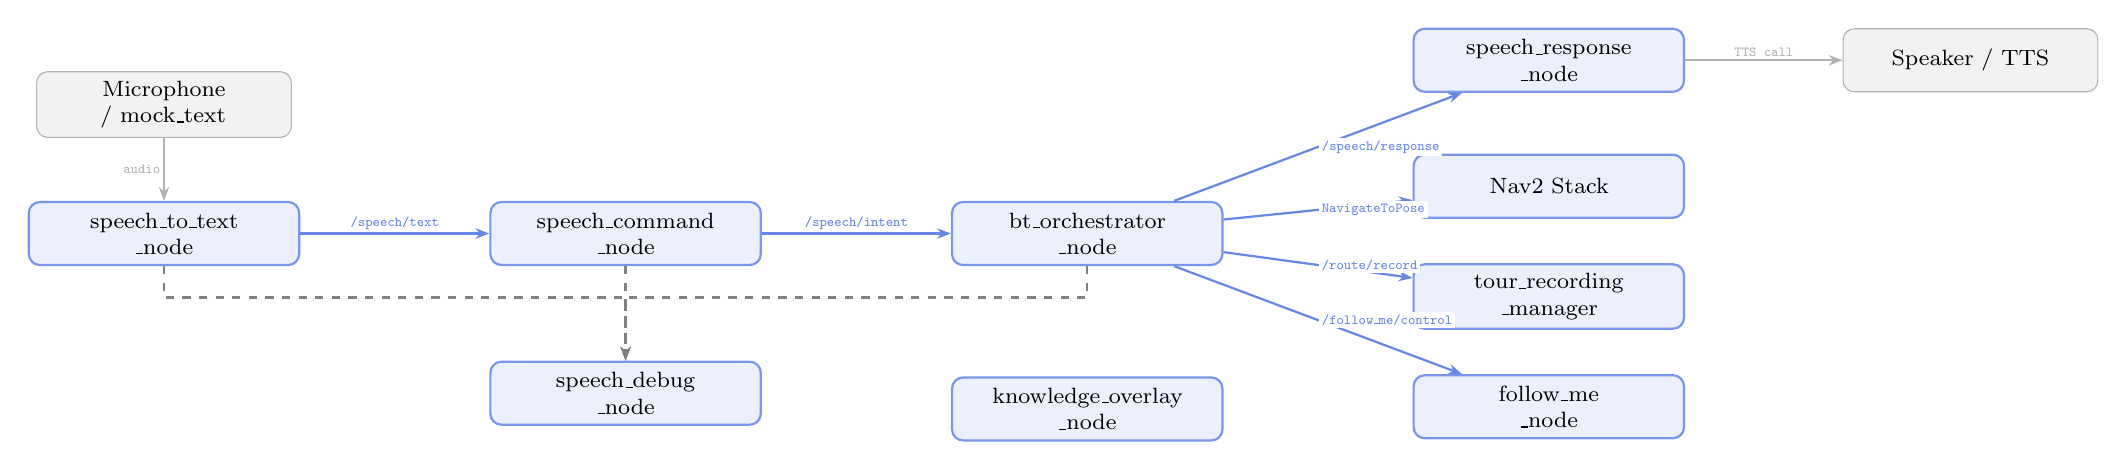
\begin{tikzpicture}[
  node distance=1.4cm and 2.2cm,
  every node/.style={font=\footnotesize},
  box/.style={rectangle, rounded corners=4pt, draw=RoyalBlue!70, fill=RoyalBlue!10,
              text width=3.2cm, align=center, minimum height=0.8cm, thick},
  extbox/.style={rectangle, rounded corners=4pt, draw=gray!60, fill=gray!10,
                 text width=3.0cm, align=center, minimum height=0.8cm},
  arrow/.style={-{Stealth[length=5pt]}, thick, RoyalBlue!80},
  garrow/.style={-{Stealth[length=5pt]}, thick, gray!60},
  label/.style={font=\tiny\ttfamily, midway, fill=white, inner sep=1pt},
]

% Column 1 — Input
\node[box] (stt)   {speech\_to\_text\\\_node};
\node[extbox, above=0.8cm of stt] (mic) {Microphone \\ / mock\_text};

% Column 2 — Command
\node[box, right=2.4cm of stt] (scn) {speech\_command\\\_node};

% Column 3 — Orchestrator
\node[box, right=2.4cm of scn] (bto) {bt\_orchestrator\\\_node};

% Column 4 — Output nodes (vertical stack)
\node[box, right=2.4cm of bto, yshift=2.2cm]  (srn)  {speech\_response\\\_node};
\node[extbox, right=2.0cm of srn]              (tts)  {Speaker / TTS};
\node[box, right=2.4cm of bto, yshift=0.6cm]  (nav2) {Nav2 Stack};
\node[box, right=2.4cm of bto, yshift=-0.8cm] (trm)  {tour\_recording\\\_manager};
\node[box, right=2.4cm of bto, yshift=-2.2cm] (fmn)  {follow\_me\\\_node};

% Debug
\node[box, below=1.2cm of scn] (sdn) {speech\_debug\\\_node};

% Knowledge
\node[box, below=1.4cm of bto] (kon) {knowledge\_overlay\\\_node};

% Arrows
\draw[garrow] (mic) -- node[label, left] {audio} (stt);
\draw[arrow] (stt) -- node[label, above] {/speech/text} (scn);
\draw[arrow] (scn) -- node[label, above] {/speech/intent} (bto);
\draw[arrow] (bto) -- node[label, right] {/speech/response} (srn);
\draw[garrow] (srn) -- node[label, above] {TTS call} (tts);
\draw[arrow] (bto) -- node[label, right] {NavigateToPose} (nav2);
\draw[arrow] (bto) -- node[label, right] {/route/record} (trm);
\draw[arrow] (bto) -- node[label, right] {/follow\_me/control} (fmn);

% Debug subscriptions (dashed)
\draw[arrow, dashed, gray] (stt.south) -- ++(0,-0.4) -| (sdn.north);
\draw[arrow, dashed, gray] (scn.south) -- ++(0,-0.4) -| (sdn.north);
\draw[arrow, dashed, gray] (bto.south) -- ++(0,-0.4) -| (sdn.north);

\end{tikzpicture}
\caption{High-level node graph (simplified; dashed lines = debug subscriptions)}
\label{fig:overview}
\end{figure}

\section{Speech Stack Data Flow}
\label{sec:speech_flow}

The speech pipeline is the most critical data path in the system.  The
sequence below describes message flow step by step:

\begin{enumerate}[leftmargin=2em]
  \item \textbf{Audio capture.}
    \node{speech\_to\_text\_node} records audio from the default
    microphone using \texttt{speech\_recognition}.  After a wake word is
    detected by \file{wake\_word.py}, it sends the audio clip to the
    Google Web Speech API (or a locally configured engine) and receives a
    plain text transcript.

  \item \textbf{Text publication.}
    The transcript is wrapped in a \texttt{std\_msgs/String} and published
    to \topic{/speech/text}.

  \item \textbf{Intent classification.}
    \node{speech\_command\_node} receives the text.  It first checks
    \file{predefined\_commands.py} for an exact or fuzzy match.  If no
    rule matches, it calls \texttt{llm\_dialogue.generate\_llm\_token()}.
    The result is a JSON intent object (see Table above) published to
    \topic{/speech/intent}.

  \item \textbf{Action dispatch.}
    \node{bt\_orchestrator\_node} receives the intent.  Based on the
    \texttt{intent} field value it:
    \begin{itemize}
      \item Sends a \texttt{NavigateToPose} goal to Nav2.
      \item Publishes control flags for tour, recording, or follow-me subsystems.
      \item Queries \file{knowledge\_store.py} and the LLM for knowledge
            questions.
      \item Publishes a response string to \topic{/speech/response}.
    \end{itemize}

  \item \textbf{Voice response.}
    \node{speech\_response\_node} receives the response string and calls
    \texttt{audio\_utils.speak()}, producing audible output.

  \item \textbf{Debug aggregation.}
    In parallel, \node{speech\_debug\_node} captures all topic messages
    and re-publishes a combined string to \topic{/speech/debug}.
\end{enumerate}

\section{Navigation and Tour Data Flow}
\label{sec:nav_flow}

\begin{enumerate}[leftmargin=2em]
  \item \textbf{Localisation.}
    In simulation, \node{sim\_initial\_pose\_node} publishes one pose to
    \topic{/initialpose}.  AMCL begins tracking from that pose using laser
    scan data.

  \item \textbf{Route recording.}
    When \node{bt\_orchestrator\_node} receives \texttt{record\_start},
    it publishes \texttt{True} to \topic{/route/record}.
    \node{tour\_recording\_manager} starts sampling \topic{/amcl\_pose}.
    The operator drives manually using \node{tour\_teleop\_session}.
    When \texttt{record\_stop} arrives, the manager publishes the waypoint
    list to \topic{/route/data}.

  \item \textbf{Tour replay.}
    \node{bt\_orchestrator\_node} reads the waypoint list and iterates
    through each waypoint, sending a separate \texttt{NavigateToPose}
    action goal for each.  The \node{talk\_at\_waypoint} Nav2 plugin
    (from \pkg{robot\_tour}) fires a speech callback at each arrival.

  \item \textbf{Person following.}
    When \topic{/follow\_me/control} becomes \texttt{True},
    \node{follow\_me\_node} activates and begins publishing to
    \topic{/cmd\_vel}, overriding Nav2.
\end{enumerate}

\section{Knowledge System Data Flow}
\label{sec:know_flow}

\begin{enumerate}[leftmargin=2em]
  \item An operator populates the SQLite database using
        \node{knowledge\_editor} (Tkinter GUI) or by importing Markdown
        files.

  \item \node{knowledge\_overlay\_node} reads location-tagged entries and
        publishes map markers to \topic{/knowledge\_markers} for display
        in RViz~2.

  \item When a visitor asks a question (intent = \texttt{explain}),
        \node{bt\_orchestrator\_node} calls
        \texttt{knowledge\_store.search(query)} to retrieve the top-$k$
        matching entries, then calls
        \texttt{llm\_dialogue.generate\_knowledge\_response()} to produce
        a grounded answer.  The answer is published to
        \topic{/speech/response}.
\end{enumerate}

%============================================================
\chapter{LLM Integration}
\label{ch:llm}
%============================================================

\section{Offline-First Design with Ollama}

All LLM inference runs \textbf{locally} through
\href{https://ollama.com}{Ollama}.  No cloud subscription, API key, or
internet connection is required.  The default model is
\texttt{qwen2.5:7b}, which runs comfortably on a laptop GPU or CPU.

\begin{table}[H]
  \centering
  \caption{LLM backend configuration}
  \begin{tabularx}{\linewidth}{L{4cm} X}
    \toprule
    \textbf{Item} & \textbf{Value} \\
    \midrule
    Engine              & Ollama (local server) \\
    Default model       & \texttt{qwen2.5:7b} \\
    Server endpoint     & \texttt{http://localhost:11434} \\
    ROS~2 parameter     & \texttt{ollama\_host}, \texttt{llm\_model} \\
    Python client       & \texttt{pip install ollama} \\
    \bottomrule
  \end{tabularx}
\end{table}

\section{Ollama Setup}

\begin{lstlisting}[style=bashstyle, caption={One-time Ollama installation and model download}]
# Install Ollama runtime
curl -fsSL https://ollama.com/install.sh | sh

# Download the model (~4 GB, done once)
ollama pull qwen2.5:7b

# Start the inference server (keep running in a separate terminal)
ollama serve

# Install the Python client library
pip install ollama
\end{lstlisting}

Other model options:

\begin{lstlisting}[style=bashstyle]
ollama pull qwen2.5:3b   # ~2 GB, faster, lower quality
ollama pull qwen2.5:14b  # ~9 GB, higher quality
\end{lstlisting}

\begin{tcolorbox}[notebox, title=No API Keys Required]
  Because Ollama runs entirely on the local machine, there are no API keys,
  no rate limits, no usage costs, and no internet dependency.
  The system works in fully air-gapped environments.
\end{tcolorbox}

\section{Fallback Behaviour}

If Ollama is not running or the \texttt{ollama} Python package is not installed,
the system falls back to rule-based intent parsing via \file{speech\_parser.py}.
Basic navigation commands continue to work without the LLM.

\section{LLM Function Reference}

\subsection{\texttt{generate\_llm\_token(utterance)}}

\textbf{Input:} Raw user utterance string.\\
\textbf{Output:} Parsed \texttt{IntentToken} with JSON-encoded intent.

The prompt instructs the LLM to return a JSON object.  Example structure:

\begin{lstlisting}[style=pythonstyle, caption={Simplified prompt sent to Ollama/Qwen}]
system_prompt = (
    "You are a robot command interpreter for a TurtleBot 3 social guide. "
    "Return strict JSON with keys: intent, label, location, response, metadata. "
    "Allowed intents: no_action, navigate, start_tour, stop, explain, ..."
)
# Ollama is called with format="json" to guarantee valid JSON output.
response = ollama_client.chat(model="qwen2.5:7b",
                              messages=messages,
                              format="json",
                              options={"temperature": 0.5})
\end{lstlisting}

\subsection{\texttt{generate\_personalized\_response(parsed)}}

\textbf{Input:} A parsed \texttt{IntentToken} with a base response.\\
\textbf{Output:} One sentence rewritten in a warm, natural tour-guide tone.

\subsection{\texttt{generate\_knowledge\_response(utterance)}}

\textbf{Input:} Visitor's spoken question.\\
\textbf{Output:} Factual answer grounded in knowledge-database content.

The function calls \texttt{KnowledgeStore.build\_context()} to assemble the
top-$k$ matching entries, then passes them as context to Ollama.
Ollama is instructed not to invent facts — it may only use the supplied context.

%============================================================
\chapter{Build, Install, and Launch}
\label{ch:build}
%============================================================

\section{Prerequisites}

Before building, ensure the following are installed:

\begin{itemize}[leftmargin=2em]
  \item ROS~2 (Humble or Iron) — source or binary installation.
  \item \texttt{colcon} — the ROS~2 build tool.
  \item Python~3.10+ with \texttt{pip}.
  \item TurtleBot~3 packages: \texttt{turtlebot3}, \texttt{turtlebot3\_gazebo}.
  \item Nav2 packages: \texttt{nav2\_bringup}, \texttt{nav2\_simple\_commander}.
\end{itemize}

Ollama and Python dependencies:

\begin{lstlisting}[style=bashstyle, caption={Installing Ollama and required Python packages}]
# Install Ollama (runs the local LLM server)
curl -fsSL https://ollama.com/install.sh | sh
ollama pull qwen2.5:7b        # download model (~4 GB, one-time)
ollama serve                  # keep this running

# Python packages
pip install ollama             # Ollama Python client (required for LLM)
pip install SpeechRecognition  # optional: microphone input
pip install opencv-python      # recommended: person-following vision
\end{lstlisting}

\section{Build Procedure}

\begin{lstlisting}[style=bashstyle, caption={Standard build procedure from workspace root}]
cd /home/karan/in_ws
colcon build
source install/setup.bash
\end{lstlisting}

\begin{tcolorbox}[notebox, title=Why source install/setup.bash?]
  \texttt{colcon build} installs the packages into the \texttt{install/}
  overlay.  The \texttt{source} command adds this overlay to the
  \texttt{AMENT\_PREFIX\_PATH}, \texttt{PYTHONPATH}, and
  \texttt{PATH} environment variables so that ROS~2 can find nodes and
  libraries by name.  This must be re-run in every new terminal session.
\end{tcolorbox}

\begin{lstlisting}[style=bashstyle, caption={Rebuild only specific packages (faster iteration)}]
colcon build --packages-select turtlebot_llm_control
source install/setup.bash
\end{lstlisting}

\section{Launch Commands}

\subsection{Full Simulation Demo}

\begin{lstlisting}[style=bashstyle, caption={Start the full Gazebo + Nav2 + Ollama simulation stack}]
# Ollama server must already be running: ollama serve
export TURTLEBOT3_MODEL=burger   # or waffle / waffle_pi
ros2 launch turtlebot_llm_control sim_pillar_nav_demo.launch.py \
  llm_model:=qwen2.5:7b \
  ollama_host:=http://localhost:11434
\end{lstlisting}

This launch file starts the following components in order:

\begin{enumerate}[leftmargin=2em]
  \item Gazebo simulator with a pillar-obstacle world.
  \item Nav2 navigation stack (AMCL + planner + controller + BT navigator).
  \item RViz~2 with the custom \file{tb3\_navigation2.rviz} configuration.
  \item \node{sim\_initial\_pose\_node} to seed AMCL.
  \item The full LLM control stack (all nodes in \pkg{turtlebot\_llm\_control}).
  \item \node{knowledge\_overlay\_node} for map markers.
  \item \node{waypoint\_visualizer} (optional) for tour waypoints.
\end{enumerate}

\subsection{Core LLM Stack Only (Hardware or Simulation)}

\begin{lstlisting}[style=bashstyle, caption={Start only the LLM control nodes}]
ros2 launch turtlebot_llm_control bringup.launch.py hardware:=false
# or for real robot hardware:
ros2 launch turtlebot_llm_control bringup.launch.py hardware:=true
\end{lstlisting}

\subsection{Individual Node Launches}

\begin{lstlisting}[style=bashstyle, caption={Run individual nodes for testing}]
# Knowledge database editor (GUI)
ros2 run turtlebot_llm_control knowledge_editor

# Manual LLM intent testing (CLI)
ros2 run turtlebot_llm_control llm_intent_test

# Speech pipeline diagnostics
ros2 run turtlebot_llm_control speech_debug_node
\end{lstlisting}

%============================================================
\chapter{Dependency Reference}
\label{ch:deps}
%============================================================

\section{ROS~2 Dependencies — \texttt{turtlebot\_llm\_control}}

\begin{longtable}{L{5cm} L{3.5cm} L{5cm}}
  \caption{ROS~2 package dependencies for \texttt{turtlebot\_llm\_control}} \\
  \toprule
  \textbf{Package} & \textbf{Type} & \textbf{Purpose} \\
  \midrule
  \endfirsthead
  \toprule
  \textbf{Package} & \textbf{Type} & \textbf{Purpose} \\
  \midrule
  \endhead
  \bottomrule
  \endfoot
  \texttt{ament\_python}        & build     & Python package build system \\
  \texttt{rclpy}                & build+run & Python ROS~2 client library \\
  \texttt{std\_msgs}            & build+run & String, Bool, Float32, etc. \\
  \texttt{std\_srvs}            & build+run & Empty, SetBool services \\
  \texttt{geometry\_msgs}       & build+run & Pose, Twist, Transform \\
  \texttt{nav\_msgs}            & build+run & OccupancyGrid, Odometry \\
  \texttt{nav2\_msgs}           & build+run & NavigateToPose action \\
  \texttt{action\_msgs}         & build+run & Action status messages \\
  \texttt{sensor\_msgs}         & build+run & Image, CompressedImage \\
  \texttt{tf2\_ros}             & build+run & Transform tree access \\
  \texttt{tf\_transformations}  & build+run & Quaternion utilities \\
  \texttt{visualization\_msgs}  & build+run & Marker, MarkerArray \\
  \texttt{launch}               & build     & Launch file infrastructure \\
  \texttt{launch\_ros}          & build     & ROS~2 launch actions \\
  \texttt{ament\_index\_python} & run       & Find installed package paths \\
  \texttt{speech\_locomotion\_interface} & run & Social guide navigation bridge \\
  \texttt{tour\_manager}        & run       & Tour save/retrieve service \\
\end{longtable}

\section{ROS~2 Dependencies — \texttt{tour\_manager}}

\begin{table}[H]
  \centering
  \caption{Dependencies for the \texttt{tour\_manager} sub-package}
  \begin{tabularx}{\linewidth}{L{4.5cm} X}
    \toprule
    \textbf{Package} & \textbf{Purpose} \\
    \midrule
    \texttt{rclpy}                   & Python ROS~2 client \\
    \texttt{geometry\_msgs}          & PoseStamped for waypoints \\
    \texttt{nav\_msgs}               & OccupancyGrid (optional) \\
    \texttt{social\_robot\_interfaces} & Tours service definition \\
    \texttt{std\_msgs}               & String messages \\
    \texttt{visualization\_msgs}     & Marker messages \\
    \bottomrule
  \end{tabularx}
\end{table}

\section{ROS~2 Dependencies — \texttt{speech\_locomotion\_interface}}

\begin{table}[H]
  \centering
  \caption{Dependencies for \texttt{speech\_locomotion\_interface}}
  \begin{tabularx}{\linewidth}{L{4.5cm} X}
    \toprule
    \textbf{Package} & \textbf{Purpose} \\
    \midrule
    \texttt{rclpy}                & Python ROS~2 client \\
    \texttt{geometry\_msgs}       & Goal pose \\
    \texttt{nav2\_simple\_commander} & High-level navigation API \\
    \texttt{std\_msgs}            & String (intent) \\
    \bottomrule
  \end{tabularx}
\end{table}

\section{Python (pip) Dependencies}

\begin{table}[H]
  \centering
  \caption{Python runtime dependencies}
  \begin{tabularx}{\linewidth}{L{4cm} L{2.5cm} X}
    \toprule
    \textbf{Library} & \textbf{Required?} & \textbf{Purpose} \\
    \midrule
    \texttt{ollama}           & \textbf{Required} & Ollama Python client for local Qwen inference \\
    \texttt{SpeechRecognition}& Optional  & Microphone-based STT \\
    \texttt{opencv-python}    & Recommended & Person-following colour tracking \\
    \texttt{tkinter}          & Standard  & Knowledge editor GUI \\
    \texttt{sqlite3}          & Standard  & Knowledge database \\
    \bottomrule
  \end{tabularx}
\end{table}

\section{System TTS Backends}

The speech response node tries these backends in order:

\begin{enumerate}[leftmargin=2em]
  \item \texttt{spd-say} — Linux Speech Dispatcher (preferred on Ubuntu).
  \item \texttt{espeak} — lighter-weight Linux TTS engine.
  \item \texttt{say} — macOS built-in TTS.
\end{enumerate}

Install on Ubuntu:
\begin{lstlisting}[style=bashstyle]
sudo apt install speech-dispatcher espeak
\end{lstlisting}

%============================================================
\chapter{Configuration Files}
\label{ch:config}
%============================================================

\section{Nav2 Parameter Files}

Three YAML files in \file{config/demo\_nav2/} configure Nav2 for different
TurtleBot~3 hardware variants.  Key parameters (tuned per-robot):

\begin{table}[H]
  \centering
  \caption{Nav2 configuration files}
  \begin{tabularx}{\linewidth}{L{3.5cm} X}
    \toprule
    \textbf{File} & \textbf{Target hardware} \\
    \midrule
    \texttt{burger.yaml}    & TurtleBot~3 Burger (smallest; differential drive) \\
    \texttt{waffle.yaml}    & TurtleBot~3 Waffle \\
    \texttt{waffle\_pi.yaml}& TurtleBot~3 Waffle Pi \\
    \bottomrule
  \end{tabularx}
\end{table}

\section{Map Files}

\begin{table}[H]
  \centering
  \caption{Demonstration map files}
  \begin{tabularx}{\linewidth}{L{4cm} X}
    \toprule
    \textbf{File} & \textbf{Description} \\
    \midrule
    \texttt{maps/demo/map.yaml} & YAML metadata: resolution, origin, occupancy thresholds \\
    \texttt{maps/demo/map.pgm}  & Greyscale PGM occupancy grid image (white = free, black = obstacle) \\
    \bottomrule
  \end{tabularx}
\end{table}

\section{RViz Configuration}

\file{rviz/tb3\_navigation2.rviz} pre-configures RViz~2 with:

\begin{itemize}[leftmargin=2em]
  \item Map display (subscribes to \topic{/map}).
  \item Robot model (subscribes to \texttt{/robot\_description}).
  \item LaserScan display (subscribes to \topic{/scan}).
  \item Navigation path and costmap overlays.
  \item MarkerArray display for knowledge points and tour waypoints.
\end{itemize}

\section{Ollama Host Configuration}

No API key file is required.  The LLM host is configured via a ROS~2 launch
argument or node parameter:

\begin{lstlisting}[style=bashstyle, caption={Configuring the Ollama endpoint}]
# Default — Ollama running on the same machine
ros2 launch turtlebot_llm_control bringup.launch.py \
  ollama_host:=http://localhost:11434 \
  llm_model:=qwen2.5:7b

# Remote Ollama server on the local network
ros2 launch turtlebot_llm_control bringup.launch.py \
  ollama_host:=http://192.168.1.50:11434 \
  llm_model:=qwen2.5:7b
\end{lstlisting}

%============================================================
\chapter{Developer Onboarding Guide}
\label{ch:onboarding}
%============================================================

\section{Recommended Reading Order}

For a developer who is new to this codebase, the following reading order
builds understanding incrementally from the simplest module to the most
complex:

\begin{enumerate}[leftmargin=2em]
  \item \textbf{\file{models.py}} — understand the data classes used everywhere.
  \item \textbf{\file{predefined\_commands.py}} — understand what hard-coded
        patterns exist.
  \item \textbf{\file{speech\_to\_text\_node.py}} — trace the entry point;
        understand wake-word gating.
  \item \textbf{\file{speech\_parser.py}} — understand rule-based parsing.
  \item \textbf{\file{llm\_dialogue.py}} — understand LLM integration and when
        it fires.
  \item \textbf{\file{speech\_command\_node.py}} — see how rules and LLM are
        combined into an intent.
  \item \textbf{\file{behavior\_tree.py}} — understand the BT primitives.
  \item \textbf{\file{bt\_orchestrator\_node.py}} — the largest file; trace
        each intent handler.
  \item \textbf{\file{tour\_recording\_manager.py}} and
        \textbf{\file{tour\_teleop\_session.py}} — tour recording pipeline.
  \item \textbf{\file{follow\_me\_node.py}} — vision-based following.
  \item \textbf{\file{knowledge\_store.py}},
        \textbf{\file{knowledge\_editor.py}},
        \textbf{\file{knowledge\_overlay\_node.py}} — knowledge subsystem.
\end{enumerate}

\section{Understanding Social Guide Integration}

The \pkg{turtlebot\_social\_guide} packages complement the main control
package in three ways:

\begin{description}[leftmargin=2em, style=nextline]
  \item[\pkg{speech\_locomotion\_interface}]
    Provides a \emph{direct path} from intent to navigation, bypassing the
    behaviour tree.  Useful for testing Nav2 independently of the BT.

  \item[\pkg{tour\_manager}]
    Hosts the tour persistence layer as a ROS~2 service, allowing other nodes
    to save and retrieve tours through a stable service interface.

  \item[\pkg{social\_robot\_interfaces}]
    Defines \texttt{Tours.srv} — the custom message type used by
    \pkg{tour\_manager}.  Always build this package first when doing a clean
    build, or use \texttt{colcon build} (which resolves build order
    automatically).
\end{description}

\section{Debugging Tips}

\begin{tcolorbox}[tipbox, title=Tip: Monitor the full speech pipeline in one command]
\begin{lstlisting}[style=bashstyle]
ros2 topic echo /speech/debug
\end{lstlisting}
\end{tcolorbox}

\begin{tcolorbox}[tipbox, title=Tip: Inject a test command without a microphone]
\begin{lstlisting}[style=bashstyle]
ros2 topic pub /speech/mock_text std_msgs/String \
  "data: 'go to the library'"
\end{lstlisting}
\end{tcolorbox}

\begin{tcolorbox}[tipbox, title=Tip: List all active topics]
\begin{lstlisting}[style=bashstyle]
ros2 topic list
ros2 node list
\end{lstlisting}
\end{tcolorbox}

\begin{tcolorbox}[tipbox, title=Tip: Test intent parsing without launching everything]
\begin{lstlisting}[style=bashstyle]
ros2 run turtlebot_llm_control llm_intent_test
\end{lstlisting}
\end{tcolorbox}

%============================================================
\chapter{Operational Procedures}
\label{ch:ops}
%============================================================

\section{First-Time Setup}

\begin{lstlisting}[style=bashstyle, caption={Complete first-time setup sequence}]
# 1. Install and start Ollama (local LLM server — no API key needed)
curl -fsSL https://ollama.com/install.sh | sh
ollama pull qwen2.5:7b          # one-time ~4 GB download
pip install ollama               # Python client library
ollama serve &                  # start server (or in a separate terminal)

# 2. Source ROS 2
source /opt/ros/humble/setup.bash

# 3. Set TurtleBot model
export TURTLEBOT3_MODEL=burger

# 4. Build workspace
cd /home/karan/in_ws
colcon build
source install/setup.bash
\end{lstlisting}

\section{Running the Simulation Demo}

\begin{lstlisting}[style=bashstyle, caption={Launch simulation in one command}]
ros2 launch turtlebot_llm_control sim_pillar_nav_demo.launch.py
\end{lstlisting}

Expected startup sequence:

\begin{enumerate}[leftmargin=2em]
  \item Gazebo opens and loads the pillar world.
  \item Nav2 initialises; AMCL awaits initial pose.
  \item \node{sim\_initial\_pose\_node} publishes the initial pose.
  \item AMCL begins localising; navigation becomes available.
  \item RViz~2 opens showing the map, robot model, and laser scan.
  \item LLM control nodes start; the robot is ready for voice commands.
\end{enumerate}

\section{Recording a Tour}

\begin{lstlisting}[style=bashstyle, caption={Start a recording session (voice commands)}]
# In a separate terminal (or speak into the microphone):
ros2 topic pub /speech/mock_text std_msgs/String "data: 'start recording'"
# Drive the robot manually using tour_teleop_session keyboard controls.
ros2 topic pub /speech/mock_text std_msgs/String "data: 'stop recording'"
# The tour is saved automatically.
\end{lstlisting}

\section{Replaying a Tour}

\begin{lstlisting}[style=bashstyle]
ros2 topic pub /speech/mock_text std_msgs/String "data: 'start tour'"
# Robot navigates through saved waypoints autonomously.
ros2 topic pub /speech/mock_text std_msgs/String "data: 'stop tour'"
\end{lstlisting}

\section{Adding Knowledge Entries}

\begin{lstlisting}[style=bashstyle]
ros2 run turtlebot_llm_control knowledge_editor
# Fill in the title, location, tags, and content fields in the GUI.
# Click Save. The entry is immediately available for LLM question answering.
\end{lstlisting}

%============================================================
\chapter{Workspace Cleanup Status}
\label{ch:cleanup}
%============================================================

The workspace has been intentionally cleaned to contain only the two production
packages.  The following items were removed during cleanup:

\begin{itemize}[leftmargin=2em]
  \item Experimental branches and prototype packages unrelated to the tour
        guide functionality.
  \item Stale \texttt{build/}, \texttt{install/}, and \texttt{log/}
        directories at the workspace root.
  \item Duplicate node implementations from earlier development iterations.
\end{itemize}

\begin{tcolorbox}[notebox, title=Clean Workspace State]
  Only two source packages remain in \texttt{src/}:
  \begin{itemize}
    \item \pkg{turtlebot\_llm\_control} — the main control package.
    \item \pkg{turtlebot\_social\_guide} — the supporting social guide package.
  \end{itemize}
  The workspace is in a buildable, deployable state as of the date of this
  document.
\end{tcolorbox}

%============================================================
\chapter{Quick-Reference Summary}
\label{ch:quickref}
%============================================================

\section{Topic Cheatsheet}

\begin{longtable}{L{5cm} L{4cm} L{4.5cm}}
  \caption{Complete topic quick reference} \\
  \toprule
  \textbf{Topic} & \textbf{Message Type} & \textbf{Producer $\to$ Consumer} \\
  \midrule
  \endfirsthead
  \toprule
  \textbf{Topic} & \textbf{Message Type} & \textbf{Producer $\to$ Consumer} \\
  \midrule
  \endhead
  \bottomrule
  \endfoot
  \topic{/speech/mock\_text}         & String           & external $\to$ stt\_node \\
  \topic{/speech/text}               & String           & stt\_node $\to$ cmd\_node \\
  \topic{/speech\_to\_text/status}   & String           & stt\_node $\to$ debug\_node \\
  \topic{/speech/intent}             & String (JSON)    & cmd\_node $\to$ bt\_node, sli \\
  \topic{/speech/response}           & String           & bt\_node $\to$ response\_node \\
  \topic{/speech/debug}              & String           & debug\_node $\to$ operator \\
  \topic{/route/record}              & Bool             & bt\_node $\leftrightarrow$ tour\_manager \\
  \topic{/save\_tour\_command}       & String           & bt\_node, teleop $\to$ tour\_manager \\
  \topic{/route/data}                & String (JSON)    & tour\_manager $\to$ bt\_node \\
  \topic{/route/replay}              & String           & bt\_node $\to$ tour\_manager \\
  \topic{/tour/status}               & String           & bt\_node, tour\_manager $\to$ operator \\
  \topic{/follow\_me/control}        & Bool             & bt\_node $\to$ follow\_me\_node \\
  \topic{/follow\_me/status}         & String           & follow\_me\_node $\to$ operator \\
  \topic{/follow\_me/debug/compressed} & CompressedImage & follow\_me\_node $\to$ RViz \\
  \topic{/manual\_override/control}  & Bool             & bt\_node $\to$ teleop\_session \\
  \topic{/reactive\_nav/control}     & Bool             & bt\_node $\to$ reactive nav \\
  \topic{/cmd\_vel}                  & Twist            & follow\_me, teleop $\to$ robot \\
  \topic{/initialpose}               & PoseWithCovarianceStamped & sim\_pose\_node $\to$ AMCL \\
  \topic{/amcl\_pose}                & PoseWithCovarianceStamped & AMCL $\to$ tour\_manager \\
  \topic{/navigate\_to\_pose}        & Action           & bt\_node $\to$ Nav2 \\
  \topic{/map}                       & OccupancyGrid    & map\_server $\to$ overlay\_node \\
  \topic{/knowledge\_markers}        & MarkerArray      & overlay\_node $\to$ RViz \\
  \topic{/visualization\_marker\_array} & MarkerArray   & waypoint\_viz $\to$ RViz \\
\end{longtable}

\section{Command Cheatsheet}

\begin{table}[H]
  \centering
  \caption{Most frequently used commands}
  \begin{tabularx}{\linewidth}{L{8cm} X}
    \toprule
    \textbf{Command} & \textbf{Effect} \\
    \midrule
    \texttt{colcon build} & Build all packages \\
    \texttt{source install/setup.bash} & Activate the workspace overlay \\
    \texttt{ros2 launch turtlebot\_llm\_control sim\_pillar\_nav\_demo.launch.py} & Full simulation demo \\
    \texttt{ros2 launch turtlebot\_llm\_control bringup.launch.py} & LLM stack only \\
    \texttt{ros2 run turtlebot\_llm\_control knowledge\_editor} & Open knowledge GUI \\
    \texttt{ros2 run turtlebot\_llm\_control llm\_intent\_test} & Test LLM intent parsing \\
    \texttt{ros2 run turtlebot\_llm\_control speech\_debug\_node} & Monitor speech pipeline \\
    \texttt{ros2 topic echo /speech/debug} & Print all speech diagnostics \\
    \texttt{ros2 topic list} & List all active topics \\
    \texttt{ros2 node list} & List all running nodes \\
    \bottomrule
  \end{tabularx}
\end{table}

%============================================================
% BIBLIOGRAPHY (placeholder — add references as needed)
%============================================================
\chapter*{References}
\addcontentsline{toc}{chapter}{References}

\begin{enumerate}[leftmargin=2em]
  \item ROS~2 Documentation. \emph{ROS~2 Humble Hawksbill}.
        \url{https://docs.ros.org/en/humble/}
  \item Nav2 Documentation. \emph{Navigation~2 — The ROS~2 Navigation Stack}.
        \url{https://navigation.ros.org/}
  \item TurtleBot~3 Documentation. \emph{ROBOTIS TurtleBot~3 Manual}.
        \url{https://emanual.robotis.com/docs/en/platform/turtlebot3/}
  \item Ollama Documentation and Model Library. \url{https://ollama.com}
  \item Qwen Model Family. \url{https://qwenlm.github.io/}
\end{enumerate}

%============================================================
% APPENDIX A — Installation and Workspace Setup
%============================================================
\appendix

\chapter{Installation and Workspace Setup}
\label{app:setup}

This appendix is a complete, sequential installation guide.
A reader following it on a clean Ubuntu~22.04 machine will reach a fully
running simulation at the end.  Every shell command is shown verbatim.

%------------------------------------------------------------
\section{Before You Start}
%------------------------------------------------------------

\subsection*{What the System Does}

\begin{itemize}[leftmargin=2em]
  \item Navigates autonomously through a mapped environment using Nav2.
  \item Listens to natural-language voice commands via a microphone.
  \item Classifies intent through a fully offline Qwen~2.5 language model
        (no internet connection required).
  \item Guides visitors on tours, speaking a prepared explanation at each stop.
  \item Answers visitor questions using Retrieval-Augmented Generation (RAG)
        over a local SQLite knowledge database.
\end{itemize}

\subsection*{Time Estimate}

\begin{tcolorbox}[notebox, title=Approximate First-Run Times]
  \begin{tabular}{ll}
    ROS~2 Humble installation  & 10--20 min (package download) \\
    TurtleBot~3 + Nav2 + Gazebo & 5--10 min \\
    Ollama + Qwen model          & 10--20 min (4.7\,GB download) \\
    Workspace build              & 2--5 min \\
    \textbf{Total}               & \textbf{30--55 min} \\
  \end{tabular}
\end{tcolorbox}

\subsection*{System Requirements}

\begin{table}[H]
  \centering
  \caption{Hardware and software requirements}
  \begin{tabularx}{\linewidth}{L{3.5cm} L{4.5cm} X}
    \toprule
    \textbf{Item} & \textbf{Minimum} & \textbf{Recommended} \\
    \midrule
    OS      & Ubuntu 22.04 LTS (x86-64) & Ubuntu 22.04 LTS (x86-64) \\
    CPU     & 4-core                    & 8-core \\
    RAM     & 8\,GB                     & 16\,GB \\
    Disk    & 20\,GB free               & 40\,GB free \\
    GPU     & Not required              & NVIDIA 6\,GB VRAM (faster LLM) \\
    Microphone & Not required           & USB cardioid mic \\
    \bottomrule
  \end{tabularx}
\end{table}

\begin{tcolorbox}[warnbox, title=Platform Compatibility]
  ROS~2 Humble has very limited support outside Ubuntu~22.04 x86-64.
  If you are on another platform (macOS, Windows, ARM, other Linux),
  install a native Ubuntu~22.04 x86-64 virtual machine before proceeding.
\end{tcolorbox}

%------------------------------------------------------------
\section{Step 1 --- Base System Packages}
%------------------------------------------------------------

Install essential build tools on a fresh Ubuntu system:

\begin{lstlisting}[style=bashstyle, caption={Base system packages}]
sudo apt update && sudo apt upgrade -y

sudo apt install -y \
  build-essential cmake git curl wget \
  python3-pip python3-venv \
  python3-tk \
  portaudio19-dev \
  libssl-dev lsb-release gnupg2 \
  software-properties-common
\end{lstlisting}

\begin{itemize}[leftmargin=2em]
  \item \file{python3-tk} --- required for the Tkinter knowledge editor GUI.
  \item \file{portaudio19-dev} --- required for microphone input via PyAudio.
\end{itemize}

%------------------------------------------------------------
\section{Step 2 --- ROS~2 Humble}
%------------------------------------------------------------

\subsection{Add the apt Repository}

\begin{lstlisting}[style=bashstyle, caption={Add the ROS~2 package repository}]
sudo curl -sSL https://raw.githubusercontent.com/ros/rosdistro/master/ros.key \
  -o /usr/share/keyrings/ros-archive-keyring.gpg

echo "deb [arch=$(dpkg --print-architecture) \
  signed-by=/usr/share/keyrings/ros-archive-keyring.gpg] \
  http://packages.ros.org/ros2/ubuntu \
  $(lsb_release -cs) main" \
  | sudo tee /etc/apt/sources.list.d/ros2.list > /dev/null

sudo apt update
\end{lstlisting}

\subsection{Install ROS~2 Desktop Full}

\begin{lstlisting}[style=bashstyle, caption={Install ROS~2 and colcon}]
sudo apt install -y ros-humble-desktop-full
sudo apt install -y python3-colcon-common-extensions python3-rosdep
\end{lstlisting}

The \texttt{desktop-full} variant includes: ROS~2 core, RViz2, \pkg{rclpy},
all standard message types, and the DDS middleware.

\subsection{Initialise rosdep}

\begin{lstlisting}[style=bashstyle, caption={Initialise rosdep}]
sudo rosdep init
rosdep update
\end{lstlisting}

\subsection{Add Sourcing to Your Shell}

\begin{lstlisting}[style=bashstyle, caption={Persistent shell sourcing}]
echo "source /opt/ros/humble/setup.bash" >> ~/.bashrc
source ~/.bashrc
\end{lstlisting}

\subsection{Verify}

\begin{lstlisting}[style=bashstyle, caption={Verify ROS~2 installation}]
ros2 --version
# Expected output: ros2 cli version X.X.X
\end{lstlisting}

%------------------------------------------------------------
\section{Step 3 --- TurtleBot~3}
%------------------------------------------------------------

\subsection{Install Packages}

\begin{lstlisting}[style=bashstyle, caption={Install TurtleBot~3 apt packages}]
sudo apt install -y \
  ros-humble-turtlebot3 \
  ros-humble-turtlebot3-msgs \
  ros-humble-turtlebot3-simulations \
  ros-humble-turtlebot3-gazebo \
  ros-humble-turtlebot3-bringup
\end{lstlisting}

\subsection{Set the Robot Model}

\begin{lstlisting}[style=bashstyle, caption={Export the robot model}]
echo "export TURTLEBOT3_MODEL=waffle" >> ~/.bashrc
source ~/.bashrc
\end{lstlisting}

\begin{table}[H]
  \centering
  \caption{TurtleBot~3 model values}
  \begin{tabular}{ll}
    \toprule
    \textbf{Value} & \textbf{When to use} \\
    \midrule
    \texttt{burger}    & Physical Burger robot \\
    \texttt{waffle}    & Simulation, or physical Waffle \\
    \texttt{waffle\_pi} & Physical Waffle Pi \\
    \bottomrule
  \end{tabular}
\end{table}

\subsection{Verify}

\begin{lstlisting}[style=bashstyle]
ros2 pkg list | grep turtlebot3
# Should list: turtlebot3, turtlebot3_gazebo, turtlebot3_msgs, ...
\end{lstlisting}

%------------------------------------------------------------
\section{Step 4 --- Nav2 Navigation Stack}
%------------------------------------------------------------

Nav2 provides localisation (AMCL), path planning, and motion control.

\begin{lstlisting}[style=bashstyle, caption={Install Nav2 packages}]
sudo apt install -y \
  ros-humble-navigation2 \
  ros-humble-nav2-bringup \
  ros-humble-nav2-simple-commander \
  ros-humble-nav2-msgs \
  ros-humble-tf-transformations
\end{lstlisting}

%------------------------------------------------------------
\section{Step 5 --- Gazebo Simulation}
%------------------------------------------------------------

Gazebo Classic (version~11) is the simulator used in the demo.

\begin{lstlisting}[style=bashstyle, caption={Install Gazebo packages}]
sudo apt install -y \
  ros-humble-gazebo-ros-pkgs \
  ros-humble-gazebo-ros2-control
\end{lstlisting}

\begin{lstlisting}[style=bashstyle, caption={Verify Gazebo}]
gazebo --version
# Expected: Gazebo multi-robot simulator, version 11.x.x
\end{lstlisting}

%------------------------------------------------------------
\section{Step 6 --- Ollama (Offline LLM)}
%------------------------------------------------------------

All language model inference runs \emph{locally} through Ollama.
No API keys, no internet connection, and no cloud account are required.

\subsection{Install Ollama}

\begin{lstlisting}[style=bashstyle, caption={Install Ollama}]
curl -fsSL https://ollama.com/install.sh | sh
\end{lstlisting}

\subsection{Start the Server}

Ollama must be running in a dedicated terminal before any ROS~2 node starts.

\begin{lstlisting}[style=bashstyle, caption={Start the Ollama inference server}]
ollama serve
\end{lstlisting}

The server listens on \texttt{http://localhost:11434}.
Leave this terminal open for the entire session.

\subsection{Download the Qwen Model}

In a \emph{second} terminal (while \texttt{ollama serve} runs in the first):

\begin{lstlisting}[style=bashstyle, caption={Pull the default model}]
ollama pull qwen2.5:7b
\end{lstlisting}

This downloads approximately 4.7\,GB once.
All subsequent starts are instant.

\begin{table}[H]
  \centering
  \caption{Model variants and hardware requirements}
  \begin{tabularx}{\linewidth}{L{3.5cm} L{2.5cm} L{3cm} X}
    \toprule
    \textbf{Model} & \textbf{Size} & \textbf{RAM needed} & \textbf{When to use} \\
    \midrule
    \texttt{qwen2.5:3b}  & $\sim$2\,GB  & 4\,GB  & Low-memory machines; fastest responses \\
    \texttt{qwen2.5:7b}  & $\sim$4.7\,GB & 8\,GB  & \textbf{Default --- best balance} \\
    \texttt{qwen2.5:14b} & $\sim$9\,GB  & 16\,GB & Higher quality reasoning \\
    \bottomrule
  \end{tabularx}
\end{table}

To use a different model pass \texttt{llm\_model:=qwen2.5:3b} at launch time.

\subsection{Install the Python Client}

\begin{lstlisting}[style=bashstyle]
pip install ollama
\end{lstlisting}

\subsection{Verify the Full Chain}

\begin{lstlisting}[style=bashstyle, caption={End-to-end Ollama verification}]
ollama run qwen2.5:7b "Say hello in one sentence."
# The model responds with a single sentence.
# Press Ctrl+D or type /bye to exit.
\end{lstlisting}

%------------------------------------------------------------
\section{Step 7 --- Speech and Audio}
%------------------------------------------------------------

\subsection{Text-to-Speech (Robot Voice Output)}

\begin{lstlisting}[style=bashstyle, caption={Install TTS backends}]
sudo apt install -y speech-dispatcher espeak
\end{lstlisting}

Test the output:

\begin{lstlisting}[style=bashstyle]
spd-say "Hello, I am your tour guide."
\end{lstlisting}

If no sound plays, check which audio sink is active:

\begin{lstlisting}[style=bashstyle]
pactl list sinks short
\end{lstlisting}

\subsection{Speech Recognition (Microphone Input)}

\begin{lstlisting}[style=bashstyle, caption={Install speech recognition dependencies}]
pip install SpeechRecognition PyAudio
\end{lstlisting}

If \texttt{PyAudio} fails to install via pip:

\begin{lstlisting}[style=bashstyle]
sudo apt install -y python3-pyaudio
\end{lstlisting}

List available microphones:

\begin{lstlisting}[style=bashstyle]
python3 -c "import speech_recognition as sr; \
            print(sr.Microphone.list_microphone_names())"
\end{lstlisting}

\begin{tcolorbox}[tipbox, title=No Microphone?]
  You can inject commands as text directly over ROS~2 topics using
  \topic{/speech/mock\_text}.  See Section~\ref{app:mock-input} for the
  exact commands.  The microphone is not required for a working demo.
\end{tcolorbox}

%------------------------------------------------------------
\section{Step 8 --- Python Packages}
%------------------------------------------------------------

\begin{lstlisting}[style=bashstyle, caption={Install all Python dependencies}]
pip install \
  ollama \
  SpeechRecognition \
  PyAudio \
  opencv-python \
  transforms3d
\end{lstlisting}

\begin{table}[H]
  \centering
  \caption{Python package purposes}
  \begin{tabularx}{\linewidth}{L{4cm} X}
    \toprule
    \textbf{Package} & \textbf{Purpose} \\
    \midrule
    \texttt{ollama}           & Offline LLM inference via local Qwen model \\
    \texttt{SpeechRecognition} & Convert microphone audio to text \\
    \texttt{PyAudio}          & Microphone access backend \\
    \texttt{opencv-python}    & Colour tracking for follow-me mode \\
    \texttt{transforms3d}     & Quaternion utilities \\
    \bottomrule
  \end{tabularx}
\end{table}

%------------------------------------------------------------
\section{Step 9 --- Build the Workspace}
%------------------------------------------------------------

\subsection{Navigate to the Workspace}

\begin{lstlisting}[style=bashstyle]
cd /home/karan/in_ws
\end{lstlisting}

\subsection{Resolve ROS Dependencies}

\begin{lstlisting}[style=bashstyle, caption={Install all ROS package dependencies}]
rosdep install --from-paths src --ignore-src -r -y
\end{lstlisting}

This reads every \file{package.xml} in \file{src/} and installs any
missing apt packages.

\subsection{Build}

\begin{lstlisting}[style=bashstyle, caption={Full workspace build}]
colcon build
\end{lstlisting}

To rebuild only the project packages after the first full build:

\begin{lstlisting}[style=bashstyle, caption={Incremental build (faster)}]
colcon build --packages-select \
  turtlebot_llm_control \
  social_robot_interfaces \
  speech_locomotion_interface \
  tour_manager \
  robot_tour
\end{lstlisting}

\subsection{Source the Overlay}

Run this in \emph{every new terminal} before using \texttt{ros2 run} or
\texttt{ros2 launch}:

\begin{lstlisting}[style=bashstyle]
source /home/karan/in_ws/install/setup.bash
\end{lstlisting}

Add it permanently to avoid forgetting:

\begin{lstlisting}[style=bashstyle]
echo "source /home/karan/in_ws/install/setup.bash" >> ~/.bashrc
source ~/.bashrc
\end{lstlisting}

\subsection{Verify}

\begin{lstlisting}[style=bashstyle]
ros2 pkg list | grep turtlebot_llm
# Expected: turtlebot_llm_control
\end{lstlisting}

%------------------------------------------------------------
\section{Step 10 --- Run the Simulation Demo}
%------------------------------------------------------------

Open \textbf{four terminals}.  Source the workspace overlay in each one.

\subsection{Terminal 1 --- Ollama Server}

\begin{lstlisting}[style=bashstyle]
ollama serve
\end{lstlisting}

Keep this running for the whole session.

\subsection{Terminal 2 --- Simulation Launch}

\begin{lstlisting}[style=bashstyle, caption={Launch the full simulation demo}]
cd /home/karan/in_ws
source install/setup.bash
export TURTLEBOT3_MODEL=waffle

ros2 launch turtlebot_llm_control sim_pillar_nav_demo.launch.py \
  enable_microphone:=true \
  llm_model:=qwen2.5:7b \
  mute:=false
\end{lstlisting}

\textbf{What to wait for} (30--60 seconds):

\begin{enumerate}[leftmargin=2em]
  \item Gazebo window opens --- robot spawns at position $(-2.0,\,-0.5)$.
  \item RViz window opens --- map loads with the pillar arena.
  \item Terminal prints \texttt{Nav2 is ready}.
  \item Terminal prints \texttt{Behavior-tree orchestrator ready}.
\end{enumerate}

\subsection{Terminal 3 --- Monitor the Speech Pipeline}

\begin{lstlisting}[style=bashstyle]
source /home/karan/in_ws/install/setup.bash
ros2 topic echo /speech/debug
\end{lstlisting}

Every spoken command, parsed intent, and robot response appears here.

\subsection{Testing Without a Microphone}
\label{app:mock-input}

Use Terminal~4 to inject text commands directly:

\begin{lstlisting}[style=bashstyle, caption={Mock speech input via ROS topic}]
source /home/karan/in_ws/install/setup.bash

# Activate the wake-word gate
ros2 topic pub --once /speech/mock_text std_msgs/String \
  "data: 'hey pepper'"

# Navigate to a location
ros2 topic pub --once /speech/mock_text std_msgs/String \
  "data: 'go to pillar 1'"

# Start a guided tour
ros2 topic pub --once /speech/mock_text std_msgs/String \
  "data: 'start tour'"

# Ask a knowledge question
ros2 topic pub --once /speech/mock_text std_msgs/String \
  "data: 'what is in this room'"
\end{lstlisting}

Monitor Terminal~3 to trace each step through the pipeline.

%------------------------------------------------------------
\section{Step 11 --- Knowledge Editor}
%------------------------------------------------------------

The knowledge editor attaches information to map locations.
When the robot arrives at a waypoint during a tour it reads the
arrival speech aloud.  Visitor questions are answered by searching
all entries (RAG).

\subsection{Open the Editor}

\begin{lstlisting}[style=bashstyle]
ros2 run turtlebot_llm_control knowledge_editor
\end{lstlisting}

The database is created automatically at:
\begin{center}
  \texttt{\textasciitilde/.local/share/turtlebot\_llm\_control/knowledge.db}
\end{center}

\subsection{Creating an Entry}

\begin{table}[H]
  \centering
  \caption{Knowledge editor field reference}
  \begin{tabularx}{\linewidth}{L{3.5cm} X}
    \toprule
    \textbf{Field} & \textbf{What to enter} \\
    \midrule
    \textbf{Key}            & Unique slug, no spaces --- e.g.\ \texttt{library}, \texttt{main\_hall} \\
    \textbf{Title}          & Human-readable name --- e.g.\ ``The Main Library'' \\
    \textbf{Kind}           & \texttt{place} for physical tour stops \\
    \textbf{X / Y}          & Map coordinates (see below for how to read them) \\
    \textbf{Yaw}            & Robot facing direction in radians (0 = East, 1.57 = North) \\
    \textbf{Arrival Speech} & Exact text the robot speaks on arrival.  Leave blank to auto-generate from the first paragraph of Wiki/Notes. \\
    \textbf{Wiki / Notes}   & Full background text used for RAG question answering. \\
    \bottomrule
  \end{tabularx}
\end{table}

Click \textbf{Save Entry} when done.

\subsection{Getting Map Coordinates}

While the simulation is running, drive the robot to the desired location
and read its pose:

\begin{lstlisting}[style=bashstyle]
ros2 topic echo /amcl_pose --once
# Read: pose.pose.position.x and pose.pose.position.y
\end{lstlisting}

Alternatively, click a point in RViz --- the coordinates appear in the
bottom status bar.

\subsection{Preview Arrival Speech}

\begin{enumerate}[leftmargin=2em]
  \item Select an entry in the list.
  \item Click \textbf{Preview Arrival Speech}.
  \item A popup shows exactly what the robot will say at that stop.
\end{enumerate}

\subsection{Test RAG Answers}

\begin{enumerate}[leftmargin=2em]
  \item Type a visitor question in the \textbf{Ask a Question} box ---
        e.g.\ ``What is special about this room?''
  \item Click \textbf{Ask}.
  \item Ollama searches the knowledge database and returns a grounded answer.
\end{enumerate}

The status bar shows \texttt{Ollama ready (model: qwen2.5:7b)} when the
LLM is connected.

%------------------------------------------------------------
\section{Step 12 --- Real Hardware Deployment}
%------------------------------------------------------------

\subsection{On the TurtleBot (Raspberry Pi)}

SSH into the robot:

\begin{lstlisting}[style=bashstyle]
ssh ubuntu@<ROBOT_IP>
\end{lstlisting}

On the robot:

\begin{lstlisting}[style=bashstyle, caption={TurtleBot bringup on the robot}]
source /opt/ros/humble/setup.bash
export TURTLEBOT3_MODEL=burger   # or waffle / waffle_pi
ros2 launch turtlebot3_bringup robot.launch.py
\end{lstlisting}

\subsection{Nav2 on the Workstation}

\begin{lstlisting}[style=bashstyle, caption={Run Nav2 on the workstation}]
export ROS_DOMAIN_ID=0    # must match the robot
source /opt/ros/humble/setup.bash
source /home/karan/in_ws/install/setup.bash
export TURTLEBOT3_MODEL=burger

ros2 launch turtlebot3_navigation2 navigation2.launch.py \
  map:=/home/karan/in_ws/src/turtlebot_LLM_control/maps/demo/map.yaml \
  use_sim_time:=false
\end{lstlisting}

\subsection{LLM Control Stack on the Workstation}

\begin{lstlisting}[style=bashstyle, caption={Run the LLM control stack}]
ros2 launch turtlebot_llm_control bringup.launch.py \
  hardware:=true \
  enable_microphone:=true \
  llm_model:=qwen2.5:7b \
  ollama_host:=http://localhost:11434
\end{lstlisting}

\subsection{Network Requirement}

Both the robot and the workstation must be on the \textbf{same Wi-Fi network}
with matching \texttt{ROS\_DOMAIN\_ID}.

\begin{lstlisting}[style=bashstyle]
export ROS_DOMAIN_ID=0
ros2 topic list    # should show /scan, /odom, /cmd_vel from the robot
\end{lstlisting}

%------------------------------------------------------------
\section{Step 13 --- Environment Variables}
%------------------------------------------------------------

Add all of the following to \texttt{\textasciitilde/.bashrc} once:

\begin{lstlisting}[style=bashstyle, caption={Complete \textasciitilde/.bashrc additions}]
# ROS 2 Humble
source /opt/ros/humble/setup.bash

# Project workspace overlay
source /home/karan/in_ws/install/setup.bash

# TurtleBot model (waffle / burger / waffle_pi)
export TURTLEBOT3_MODEL=waffle

# Gazebo model path for TurtleBot 3
export GAZEBO_MODEL_PATH=$GAZEBO_MODEL_PATH:/opt/ros/humble/share/turtlebot3_gazebo/models
\end{lstlisting}

Apply immediately:

\begin{lstlisting}[style=bashstyle]
source ~/.bashrc
\end{lstlisting}

%------------------------------------------------------------
\section{Step 14 --- Launch Arguments Reference}
%------------------------------------------------------------

\subsection{\texttt{sim\_pillar\_nav\_demo.launch.py} (Simulation)}

\begin{table}[H]
  \centering
  \caption{Launch arguments for the full simulation demo}
  \begin{tabularx}{\linewidth}{L{5.5cm} L{3.5cm} X}
    \toprule
    \textbf{Argument} & \textbf{Default} & \textbf{Description} \\
    \midrule
    \texttt{enable\_microphone}  & \texttt{true}  & Enable live microphone input \\
    \texttt{enable\_llm}         & \texttt{true}  & Use Ollama; \texttt{false} = rules only \\
    \texttt{llm\_model}          & \texttt{qwen2.5:7b} & Ollama model name \\
    \texttt{ollama\_host}        & \texttt{http://localhost:11434} & Ollama server address \\
    \texttt{knowledge\_db\_path} & (auto) & SQLite database path override \\
    \texttt{mute}                & \texttt{false} & Silence all TTS output \\
    \texttt{enable\_speech\_debug} & \texttt{true} & Start the pipeline aggregator node \\
    \texttt{enable\_knowledge\_editor} & \texttt{false} & Launch the editor alongside the robot \\
    \texttt{enable\_direct\_locomotion\_interface} & \texttt{false} & Direct speech $\to$ Nav2 bridge \\
    \texttt{tour\_db\_path}      & (auto) & Tour waypoint database path override \\
    \bottomrule
  \end{tabularx}
\end{table}

\subsection{\texttt{bringup.launch.py} (Hardware or Simulation)}

All arguments from Table~A.5 apply, plus:

\begin{table}[H]
  \centering
  \caption{Additional argument for \texttt{bringup.launch.py}}
  \begin{tabularx}{\linewidth}{L{3cm} L{2.5cm} X}
    \toprule
    \textbf{Argument} & \textbf{Default} & \textbf{Description} \\
    \midrule
    \texttt{hardware} & \texttt{false} & \texttt{true} = real robot (disables sim time) \\
    \bottomrule
  \end{tabularx}
\end{table}

%------------------------------------------------------------
\section{Troubleshooting}
%------------------------------------------------------------

\subsection{Ollama Not Responding}

\begin{lstlisting}[style=bashstyle]
curl http://localhost:11434/api/tags
\end{lstlisting}

If this fails, start the server:

\begin{lstlisting}[style=bashstyle]
ollama serve
\end{lstlisting}

If the model is missing:

\begin{lstlisting}[style=bashstyle]
ollama list                # see what is downloaded
ollama pull qwen2.5:7b    # re-download if needed
\end{lstlisting}

\subsection{Robot Does Not Speak}

\begin{lstlisting}[style=bashstyle]
which spd-say && spd-say "test"
which espeak  && espeak "test"
\end{lstlisting}

Install TTS if missing:

\begin{lstlisting}[style=bashstyle]
sudo apt install -y speech-dispatcher espeak
\end{lstlisting}

Publish a test message directly to the TTS node:

\begin{lstlisting}[style=bashstyle]
ros2 topic pub --once /speech/response std_msgs/String "data: 'hello'"
\end{lstlisting}

\subsection{Nav2 Does Not Accept Goals}

Check the initial pose was published:

\begin{lstlisting}[style=bashstyle]
ros2 topic echo /initialpose --once
\end{lstlisting}

Publish it manually if nothing appears:

\begin{lstlisting}[style=bashstyle]
ros2 topic pub --once /initialpose \
  geometry_msgs/PoseWithCovarianceStamped \
  "{header: {frame_id: 'map'}, \
    pose: {pose: {position: {x: -2.0, y: -0.5, z: 0.0}, \
                  orientation: {w: 1.0}}}}"
\end{lstlisting}

\subsection{\texttt{colcon build} Fails with Missing Packages}

\begin{lstlisting}[style=bashstyle]
cd /home/karan/in_ws
rosdep install --from-paths src --ignore-src -r -y
colcon build
\end{lstlisting}

\subsection{\texttt{ModuleNotFoundError: No module named 'ollama'}}

\begin{lstlisting}[style=bashstyle]
pip install ollama
python3 -c "import ollama; print('OK')"
\end{lstlisting}

\subsection{Intent Always Returns \texttt{no\_action}}

\begin{enumerate}[leftmargin=2em]
  \item Verify Ollama is reachable: \texttt{curl http://localhost:11434/api/tags}
  \item Check \node{speech\_command\_node} logs --- it prints \texttt{client=True}
        on startup when the connection succeeds.
  \item Watch \topic{/speech/debug} to see the raw text and parsed intent.
  \item Run the interactive LLM test tool:
\end{enumerate}

\begin{lstlisting}[style=bashstyle]
ros2 run turtlebot_llm_control llm_intent_test
\end{lstlisting}

\subsection{Knowledge Editor Window Does Not Open}

\begin{lstlisting}[style=bashstyle]
python3 -c "import tkinter; tkinter._test()"
sudo apt install -y python3-tk
\end{lstlisting}

\subsection{Gazebo Is Very Slow or Crashes}

\begin{lstlisting}[style=bashstyle]
export SVGA_VGPU10=0    # disable GPU renderer (useful in VMs)
ros2 launch turtlebot_llm_control sim_pillar_nav_demo.launch.py \
  enable_microphone:=false mute:=true
\end{lstlisting}

%------------------------------------------------------------
\section{Quick-Start Checklists}
%------------------------------------------------------------

\subsection*{Pre-Session Checklist (before every demo)}

\begin{itemize}[leftmargin=2em, label=$\square$]
  \item \texttt{ollama serve} is running in a dedicated terminal.
  \item \texttt{ollama list} shows \texttt{qwen2.5:7b}.
  \item \texttt{TURTLEBOT3\_MODEL} is exported in the launch terminal.
  \item \texttt{source install/setup.bash} has been run in the launch terminal.
  \item \texttt{colcon build} completed with no errors since the last code change.
  \item At least one knowledge entry with X/Y coordinates is saved.
\end{itemize}

\subsection*{Full One-Time Setup Checklist}

\begin{itemize}[leftmargin=2em, label=$\square$]
  \item Ubuntu 22.04 LTS (x86-64) installed.
  \item \texttt{ros-humble-desktop-full} installed and sourced.
  \item \texttt{python3-colcon-common-extensions} installed.
  \item TurtleBot~3 apt packages installed.
  \item Nav2 apt packages installed.
  \item Gazebo apt packages installed.
  \item Ollama installed (\texttt{ollama --version} succeeds).
  \item \texttt{ollama pull qwen2.5:7b} completed.
  \item \texttt{pip install ollama} completed.
  \item \texttt{pip install SpeechRecognition PyAudio opencv-python transforms3d}
        completed.
  \item \texttt{sudo apt install speech-dispatcher espeak} completed.
  \item \texttt{rosdep install --from-paths src --ignore-src -r -y} run.
  \item \texttt{colcon build} succeeded with no errors.
  \item \texttt{source /opt/ros/humble/setup.bash} added to \texttt{\textasciitilde/.bashrc}.
  \item \texttt{source /home/karan/in\_ws/install/setup.bash} added to
        \texttt{\textasciitilde/.bashrc}.
  \item \texttt{export TURTLEBOT3\_MODEL=waffle} added to
        \texttt{\textasciitilde/.bashrc}.
  \item \texttt{export GAZEBO\_MODEL\_PATH=\ldots} added to
        \texttt{\textasciitilde/.bashrc}.
\end{itemize}

%============================================================
\end{document}
%============================================================
